\chapter{EXPERIMENTAL SETUP}
\label{EXPERIMENTAL SETUP}

The Q-weak experiment (E08-016) was performed at Thomas Jefferson National Accelerator Facility (TJNAF)~\cite{website:jlab} in Newport News, Virginia from January 2011 to May 2012~\cite{qweak_proposal_2001, qweak_proposal_2004, qweak_proposal_2007}. 
The goal of the Q-weak experiment is to extract the weak charge of the proton by measuring parity violating (\newnot{symbol:PV}PV) asymmetry in elastic electron-proton scattering at low momentum transfer. The Standard Model (\newnot{symbol:SM}SM) predicts this asymmetry to be $\sim-$250~parts per billion (\newnot{symbol:ppb}ppb) and the Q-weak collaboration proposed to measure this asymmetry with 2.1\% statistical uncertainty. The Q-weak experiment has highly benefited from technologies developed by previous parity violating experiments such as SAMPLE~\cite{Beise2005289} at the MIT/Bates Linear Accelerator Center, G0~\cite{PhysRevLett.95.092001} and HAPPEX~\cite{PhysRevLett.96.022003} at JLab. As the Q-weak PV asymmetry and its absolute uncertainty are an order of magnitude smaller than its predecessors, a dedicated design, significant improvement to hardware and software, and additional control of systematic uncertainties were needed to reach the proposed precision goals summarized in Table~\ref{tab:qweak_proposal}. A brief description of the experimental setup will be discussed in this chapter.

\begin{singlespace}
\begin{table}[!h]
\begin{center}
  	\caption
%  	[Proposed error budget of the Q-weak experiment.]
  	{Proposed error budget of the Q-weak experiment \cite{qweak_proposal_2007}. The second and third columns show the relative uncertainty on parity violating asymmetry, and on weak charge of proton, respectively. Total uncertainty is the quadrature sum of the statistical and systematic uncertainty.}
  \begin{tabular}{ l | c | c }
%    \hline
    \noalign{\hrule height 1pt}
    Source of Error & $\displaystyle\frac{\Delta A_{PV}}{A_{PV}}$ & $\displaystyle\frac{\Delta Q_{W}^{p}}{Q_{W}^{p}}$\\ 
%    \hline
    \noalign{\hrule height 1pt}
	Statistics & 2.1\% & 3.2\%\\
	Hadronic structure & - & 1.5\%\\
	Beam polarization & 1.0\% & 1.5\%\\
	Absolute $Q^{2}$ & 0.5\% & 1.0\%\\
	Backgrounds & 0.7\% & 0.7\%\\
	Helicity correlated beam properties & 0.5\% & 0.8\%\\ \hline
	Total & 2.6\% & 4.2\%\\
%    \hline
    \noalign{\hrule height 1pt}
  	\end{tabular}
  \label{tab:qweak_proposal}
\end{center}
\end{table}
\end{singlespace}



%%%%%%%%%%%%%%%%%%%%%%%%%%%%%%%%%%%%%%%%%%%%%%%%%%%%%%%%%%%%%%%%%%%%%%%
\section{Q-weak Kinematics\index{Q-weak!Kinematics}}%
\label{Q-weak Kinematics}

\begin{singlespace}
\begin{figure}[!h]
	\begin{center}
	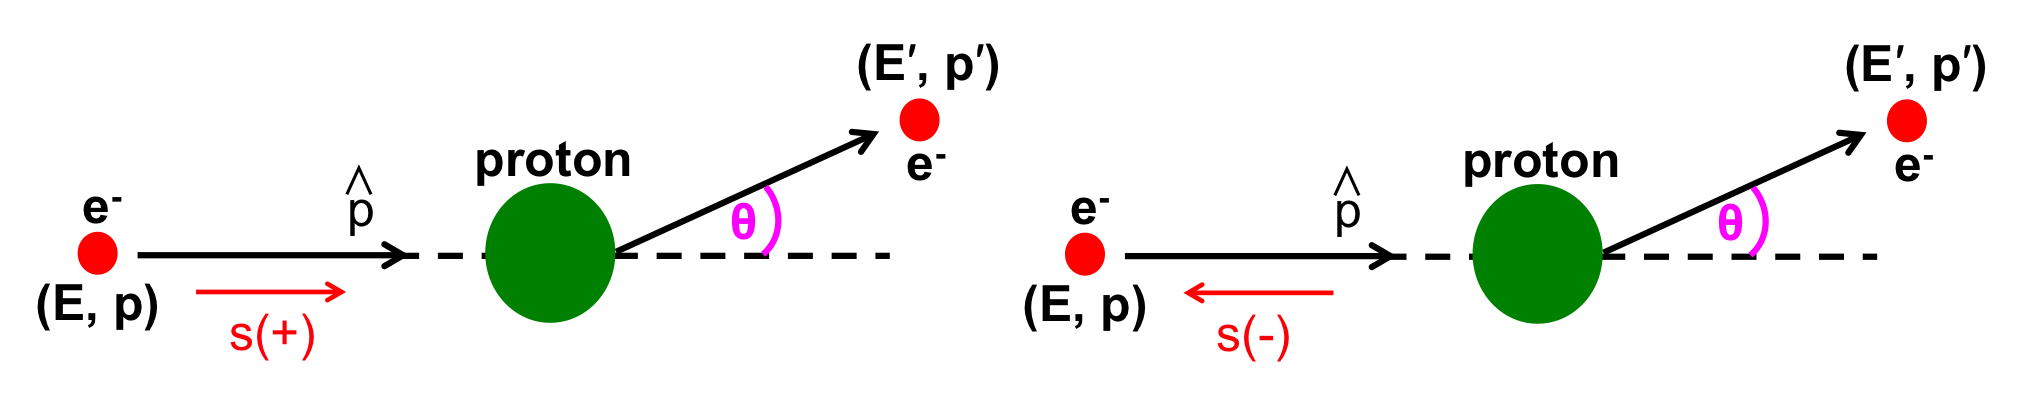
\includegraphics[width=15.0cm]{figures/e+p_scattering}
	\end{center}
	\caption
%	[Sketch of the elastic electron-proton scattering process.]
	{Sketch of the elastic electron-proton scattering process. An electron with energy ($E$) and momentum ($p$) scatters off a proton conserving the total energy of the system. $E^{\prime}$ and $p^{\prime}$ are the energy and momentum of the electron after scattering. The $+$ helicity is denoted as the projection of the electron spin $S$ along the direction of the momentum (shown in left), whereas $-$ helicity is the projection of the spin opposite to the direction of the momentum (shown in right).}
	\label{fig:e-p_scattering}
\end{figure}
\end{singlespace}

In two-body elastic electron-proton scattering, an incident electron with energy $E$ and momentum $p$ scatters from a stationary proton with mass $M$. The electron scatters with energy $E^{\prime}$ and momentum $p_{0}$ at an angle $\theta$ with respect to the incident electron as shown in Figure~\ref{fig:e-p_scattering}. The energy transfer can be expressed as $\nu = E - E^{\prime}$ and 3-momentum transfer as $\textbf{q}$ = $\textbf{p}$ - $\textbf{p}^{\prime}$. Then the four momentum transfer can be defined as 

\begin{equation} \label{equ:kinQ2_1}
Q^{2} = -q^{2} = -(\nu^{2} - \textbf{q}^{2}) \geq 0
\end{equation}

Using energy and momentum conservation for two-body scattering, the scattered energy $E^{\prime}$ and $Q^{2}$ can be written as

\begin{equation} \label{equ:kinEprime}
E^{\prime} = \frac{E}{ 1 + 2\frac{E}{M}\sin^{2} \frac{\theta}{2} }
\end{equation}

\begin{equation} \label{equ:kinQ2}
Q^{2} = \frac{4E^{2}\sin^{2}\frac{\theta}{2}}{ 1 + 2\frac{E}{M}\sin^{2}\frac{\theta}{2} }.
\end{equation}

A dedicated tracking system was used to measure the scattering angle $\theta$ and $Q^{2}$ 
%to improve simulation
 (more details in Section~\ref{Tracking Detector System}). Simulation was used to confirm measurements. 
A longitudinally polarized electron beam with energy 1.155~GeV was incident on 34.4~cm long liquid hydrogen target (\newnot{symbol:LH$_{2}$}LH$_{2}$) where a magnetic spectrometer selected out the elastic electron-proton scattering at $Q^{2}$ $\sim$0.025~(GeV/c)$^{2}$. A summary of the basic parameters and typical operating conditions for the experiment are shown in Table~\ref{tab:qweak_kinematics}. The design parameters of the experiment were chosen to minimize the contributions from the anticipated systematic uncertainties shown in Table~\ref{tab:qweak_proposal}.

\begin{singlespace}
\begin{table}[!h]
\begin{center}
  	\caption
%  	[Basic parameters and typical operating conditions of the Q-weak experiment.]
  	{Basic parameters and typical operating conditions of the Q-weak experiment~\cite{qweak_proposal_2007,qweak25percent,nur_qweak_ICNFP_paper}.}
  \begin{tabular}{ l | c }
%    \hline
    \noalign{\hrule height 1pt}
	Parameter & Value\\ 
%	\hline
    \noalign{\hrule height 1pt}
	Incident beam energy & 1.155~GeV\\
	Beam polarization & 89\%\\
	Beam current & 180~$\mu$A\\
	LH$_{2}$ target thickness & 34.4~cm \\
	Cryopower & 2.5~kW\\
	Production running time & 2544~hours\\
	Nominal scattering angle & 7.9\degrees{} \\
	Scattering angle acceptance & $\pm$3\degrees{} \\
	Acceptance & 49\% of 2$\pi$\\
	Solid angle & $\Delta \Omega$ = 43~msr\\
	Acceptance averaged $Q^{2}$ & $\langle Q^{2}\rangle$ = 0.025~(GeV/c)$^{2}$\\
	Acceptance averaged physics asymmetry & $\langle A \rangle$ = -234~ppb\\
	Acceptance averaged experimental asymmetry & $\langle A \rangle$ = -200~ppb\\
	Luminosity & 2$\times$10$^{39}$~s$^{-1}$cm$^{-2}$\\
	Integrated cross section & 4.0~$\mu$b\\
	Integrated rate (all sectors) & 6.5~GHz (0.81~GHz per sector)\\
	Full Current Production Running & 2544~hours\\
%    \hline
    \noalign{\hrule height 1pt}
  	\end{tabular}
  \label{tab:qweak_kinematics}
\end{center}
\end{table}
\end{singlespace}


\begin{singlespace}
\begin{figure}[!h]
	\begin{center}
	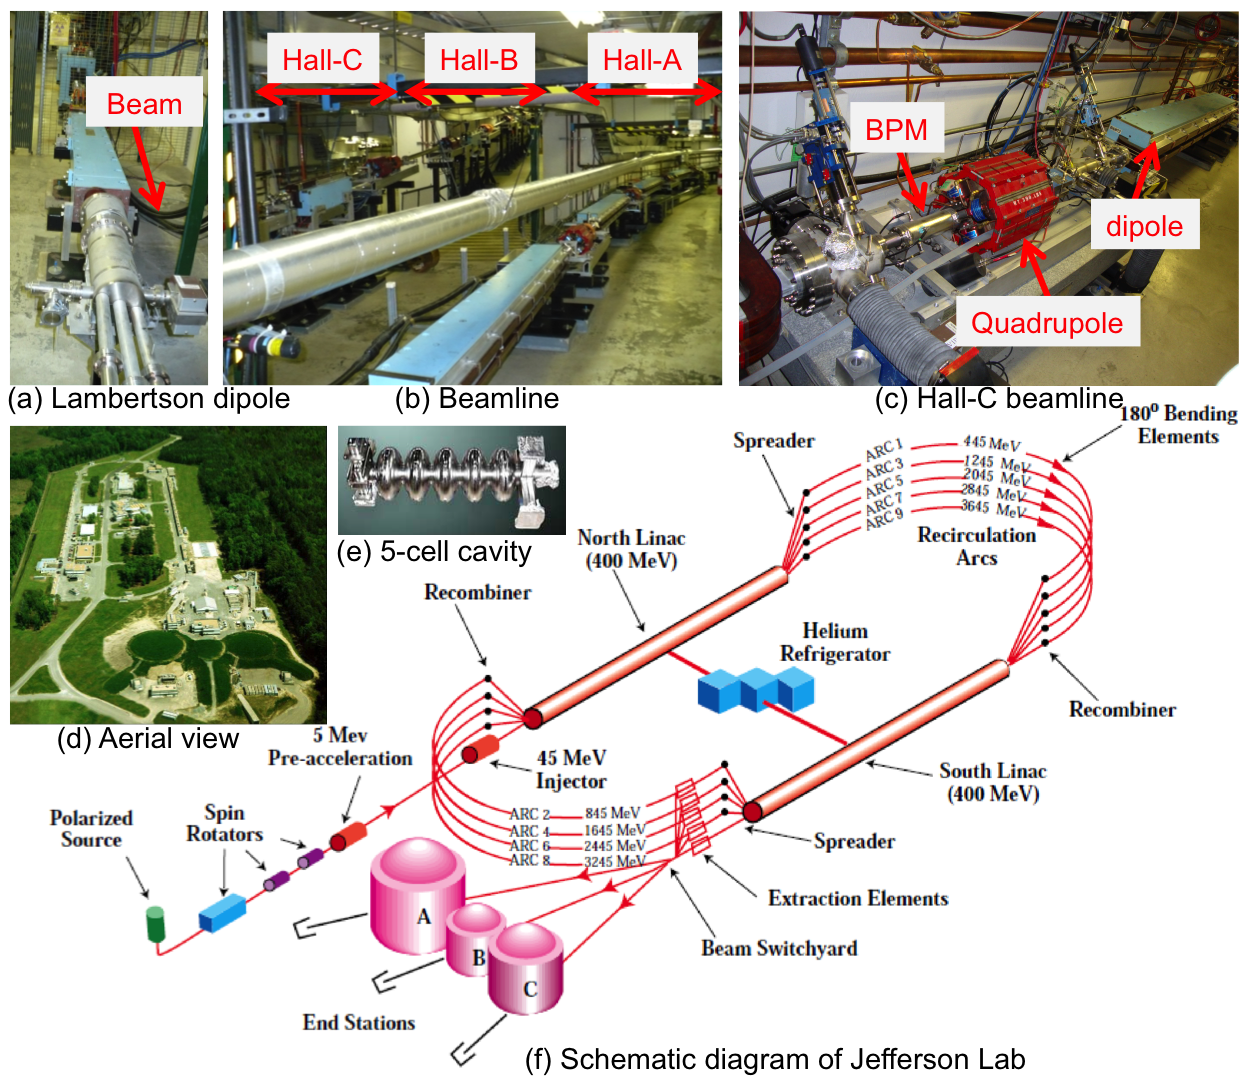
\includegraphics[width=15.0cm]{figures/jlab}
	\end{center}
	\caption
%	[Jefferson Lab and its beamline schematic.]
	{Jefferson Lab and its beamline schematic. (a) Dipole at Lambertson region where beam splits for three different experimental halls. (b) Three separate beamlines for three halls. (c) Hall-C beamline before entering in the hall. A typical quadrupole, dipole, and BPM are shown. (d) Aerial view of Jefferson Lab. (e) A JLab made 5-cell accelerating cavity. (f) Schematic diagram of Jefferson Lab. The elliptical region is the electron accelerator. Beam is accelerated by two linear accelerator namely North and South linac in the straight sections. Three existing Halls A, B, C are shown.}
	\label{fig:jlab}
\end{figure}
\end{singlespace}

%%%%%%%%%%%%%%%%%%%%%%%%%%%%%%%%%%%%%%%%%%%%%%%%%%%%%%%%%%%%%%%%%%%%%%%
\section{Experimental Techniques}%
\label{Experimental Techniques}

The parity-violating asymmetry is defined as the difference over sum of the cross section for two different helicity states (+/-) as shown in Equation~\ref{equ:asymmetryDefinition}. The helicity state of the longitudinally polarized electron beam is flipped between ``+" and ``-" and scattered off from a fixed un-polarized proton target. The signal from elastically scattered electron for each helicity state is integrated to measure the yield ($Y^{+/-}$). The difference in helicity correlated yield is sensitive to parity violating quantities. The raw asymmetry extracted from helicity correlated yields is defined as

\begin{equation} \label{equ:asymmetryDefinition}
A_{\textrm{raw}} = \frac{Y^{+}-Y^{-}}{Y^{+}+Y^{-}} \propto \frac{\displaystyle \left(\frac{d\sigma}{d\Omega}\right)^{+} - \left(\frac{d\sigma}{d\Omega}\right)^{-} }{\displaystyle \left(\frac{d\sigma}{d\Omega}\right)^{+} + \left(\frac{d\sigma}{d\Omega}\right)^{-}}.
\end{equation}

The electron beam polarization was changed pseudo-randomly in a quartet (QRT) pattern of either ``+ - - +" or``- + + -" with a helicity reversal rate of 960~Hz. The combination of fast helicity reversal and pseudo-random QRT patterns cancel the slow drifts in yields, and minimizes the target density fluctuations. Any common scale factors between the two helicity states cancel, but any difference does not. Hence Helicity Correlated Beam Asymmetries (HCBAs) in beam parameters like position, angle, energy, and charge can generate false asymmetries in measured asymmetry. Linear regression based on natural beam jitter or driven beam modulation is used to correct for such false asymmetries. The asymmetry is then corrected for the beam polarization, several background contributions, and various experimental biases to obtain the final party violating asymmetry.


%%%%%%%%%%%%%%%%%%%%%%%%%%%%%%%%%%%%%%%%%%%%%%%%%%%%%%%%%%%%%%%%%%%%%%%
%\section{\newnot{symbol:TJNAF}TJNAF\index{TJNAF} Overview}%
\section{TJNAF\index{TJNAF} Overview}%
\label{TJNAF}

The electron accelerator in \newnot{symbol:TJNAF}TJNAF or Jefferson Lab (\newnot{symbol:JLab}JLab) is known as the Continuous Electron Beam Accelerator Facility 
%(CEBAF\index{CEBAF})
(\newnot{symbol:CEBAF}CEBAF\index{CEBAF})~\cite{Leemann_CEBAF}, uses superconducting radio frequency (\newnot{symbol:SRF}SRF) technology to accelerate electrons up to 6~GeV and is capable of simultaneous beam delivery to all three experimental halls (A, B and C) at different energies, beam intensities, and orientation of beam polarization. The Q-weak experiment was carried out in the experimental Hall-C during January 2011 to May 2012, although preparation began in 2001. In the future, JLab will upgrade its energy from 6~GeV to 12~GeV, and a new experimental hall (Hall-D) will be added~\cite{website:jlab_12GeV}. A schematic of CEBAF is shown in Figure~\ref{fig:jlab} (f). The JLab electron beam starts from a polarized source and end in the beam dump at the end station. The longitudinally polarized beam starts from the source and travels through a series of spin rotators and then accelerated by two linear accelerators and enter the experimental Hall-C. Throughout the beamline, quadrupoles and dipoles were used to focus/defocus the beam and beam position monitors (\newnot{symbol:BPM}BPMs), and beam current monitors (\newnot{symbol:BCM}BCMs) were used to track the beam at any given point along the beamline. 
Polarimeters were used to measure the beam polarization before the hall entrance. 
Inside Hall-C there were various modules of the experimental apparatus like targets, collimators, toroidal magnet, and detectors.
This chapter will discuss various key components of the experimental apparatus in following subsections.

\begin{singlespace}
\begin{figure}[!h]
	\begin{center}
	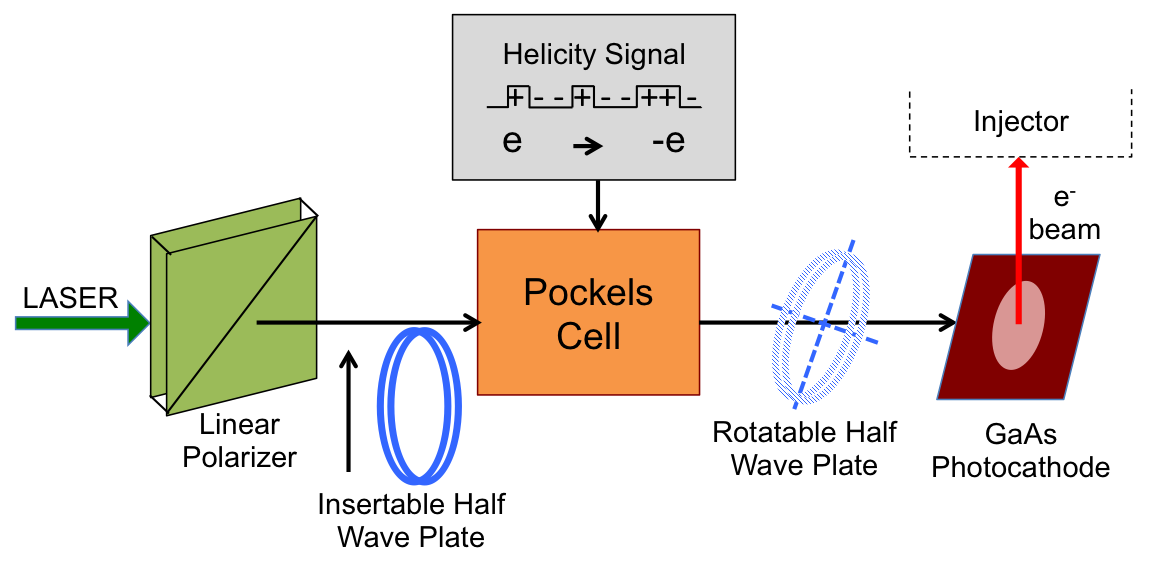
\includegraphics[width=15.0cm]{figures/source}
	\end{center}
	\caption
%	[Schematic showing the process of producing circularly polarized light.]
	{Schematic showing the process of producing circularly polarized light. The LASER is circularly polarized before GaAs photocathode using Pockels cell.}
	\label{fig:source}
\end{figure}
\end{singlespace}


\subsection{Polarized Source\index{Polarized Source} and Helicity Reversal\index{Helicity Reversal}}%
\label{Polarized Source and Helicity Reversal}

The production of the electron beam starts with the polarized electron source. Circularly polarized\index{Polarized Source!Circularly polarized} light is used to produce polarized electrons from a strained super-lattice Gallium-Arsenide (GaAs\index{Polarized Source!GaAs}) cathode via the photo-electric effect. This cathode is composed of several layers of material containing GaAs with varying amounts of phosphorus doping, grown on a substrate. 
Supperlattice structure (alternating layers of GaAs and strained GaAs) increased the quantum efficiency (\newnot{symbol:QE}QE), which is the probability of the electron emission per photon~\cite{presentation:poelker_source_1436}.
Each experimental hall has a dedicated laser that emits light at 1560 nm and pulses are 120\degrees{} out of phase in order to provide beam delivery in all halls simultaneously. To ensure total linear polarization,  the light was passed through linear polarizers (shown in Figure~\ref{fig:source}). 
An insertable half wave plate (\newnot{symbol:IHWP}IHWP) was used to flip the relative direction of the linearly polarized light without changing electronic helicity signal, which helps to isolate false asymmetry effects. IHWP changes the spin of the electrons by 180\degrees{}, this provided two independent data sets namely IHWP-IN and IHWP-OUT, that helped remove further helicity correlated beam asymmetries (\newnot{symbol:HCBA}HCBA). IHWP states were changed at a time interval of eight hours, called slugs. A Pockels cell was used to convert linearly polarized light to circularly polarized electrons using induced birefringence. Just after the Pockels cells, a rotatable half wave plate (\newnot{symbol:RHWP}RHWP) was used to rotate the residual linear polarization to circular polarization. This also helps minimize the effect due to the helicity-correlated beam parameters that arise from the residual linear polarization interacting with the photocathode.
A more detailed overview of polarized electron beam technology with references to the scientific literature on the subject is available in \cite{jlab_source_book}.

A double Wien filter was used to rotate the polarization of the electron beam in order to fine tune and produce fully longitudinally polarized beam during the experiment \cite{grames_double_wien_proceedings}. A single Wien system can flip the polarization of the beam by 90\degrees{}. In a double Wien system both Wiens can rotate polarization by 90\degrees{} which help to cancel systematic false asymmetries. This method also helped to produce fully transversely polarized beam for ancillary and background measurements. A dedicated chapter on transverse polarization measurement will be discussed later.


%%%%%%%%%%%%%%%%%%%%%%%%%%%%%%%%%%%%%%%%%%%%%%%%%%%%%%%%%%%%%%%%%%%%%%%
\section{Accelerator\index{Accelerator}}%
\label{Accelerator}

The length of the accelerator is about 7/8~miles for one complete cycle. A thermionic electron gun is used as the source of electron at the injector to extract electron beam of energy 67~MeV with the standard setup. 
The electron beam is accelerated by two linear accelerators (\newnot{symbol:linac}linacs), north and south linacs. A series of magnets bends the beam along the arcs which connects the two linacs. The beamlines, transporting the beam to the three halls are shown in the Figure~\ref{fig:jlab} (f) by the red lines. 
Electrons from the injector are sent to the north \newnot{symbol:linac}linac at an energy of 67~MeV. Superconducting niobium RF resonant cavities shown in Figure~\ref{fig:jlab} (e) in the north linac section accelerate the electrons, in a standard tune the maximum gain in energy per linac is 600~MeV. There are 20 cryomodules per linac, where each cryomodule consists of 8 cavities with an outer vacuum vessel, thermal radiation shield, magnetic shield, super insulation, and a welded helium vessel ~\cite{Leemann_CEBAF,kmyers_qweak}. The beam then goes through the east arc and into the south linac to accelerate for another 600~MeV energy gain. This beam can be sent directly to the Beam Switch Yard (\newnot{symbol:BSY}BSY) for distribution to the experimental halls (Figure~\ref{fig:jlab} (a)) or the beam can be steered along the west arc for another pass through the two linacs for another 1.2~GeV of energy gain. This process can be repeated up to four times. A maximum of five passes  through both linacs provide energies from 445~MeV to 5945~MeV. As the beam energies are different in each passs, a different set of magnets are used to steer the beam around the arcs after each pass. One pass beam was used for the Q-weak experiment as the required beam energy was 1.155~GeV.

%%%%%%%%%%%%%%%%%%%%%%%%%%%%%%%%%%%%%%%%%%%%%%%%%%%%%%%%%%%%%
\section{Beamline\index{Beamline}}%
\label{Beamline}

The beamlines that transport the beam from the accelerator to the experimental halls are shown in Figure~\ref{fig:jlab}. A two meter long dipole splits the beam for three different halls at Lambertson (Figure~\ref{fig:jlab} (a)). Beamlines for each hall (Figure~\ref{fig:jlab} (b)) consists of a series of quadrupole and dipole magnets to transport the beam to the target in each hall (shown in Figure~\ref{fig:jlab} (c) for Hall-C). Total length of Hall-C beamline from the Lambertson to the beam dump was 196.12~m.
The beam position, profile and current were measured at various points along the beamline using BPMs (Figure~\ref{fig:jlab} (c)) and BCMs, respectively. A part of Hall-C beamline also forms an arc, the bending magnets of the Hall-C arc were used to measure the relative beam energy with a precision of $\Delta$E/E $\approx$ $10^{-4}$ (details in Section~\ref{Beam Energy}).
A details sketch of Hall-C beamline elements is provided in APPENDIX~\ref{BEAM MODULATION 2} and discussed in technical document~\cite{nur_beamline_sketch}.

%%%%%%%%%%%%%%%%%%%%%%%%%%%%%%%%%%%%%%%%%%%%%%%%%%%%%%%%%%%%%
\section{Beam Monitoring\index{Beam Monitoring}}%
\label{Beam Monitoring}

\begin{singlespace}
\begin{figure}[!h]
	\begin{center}
	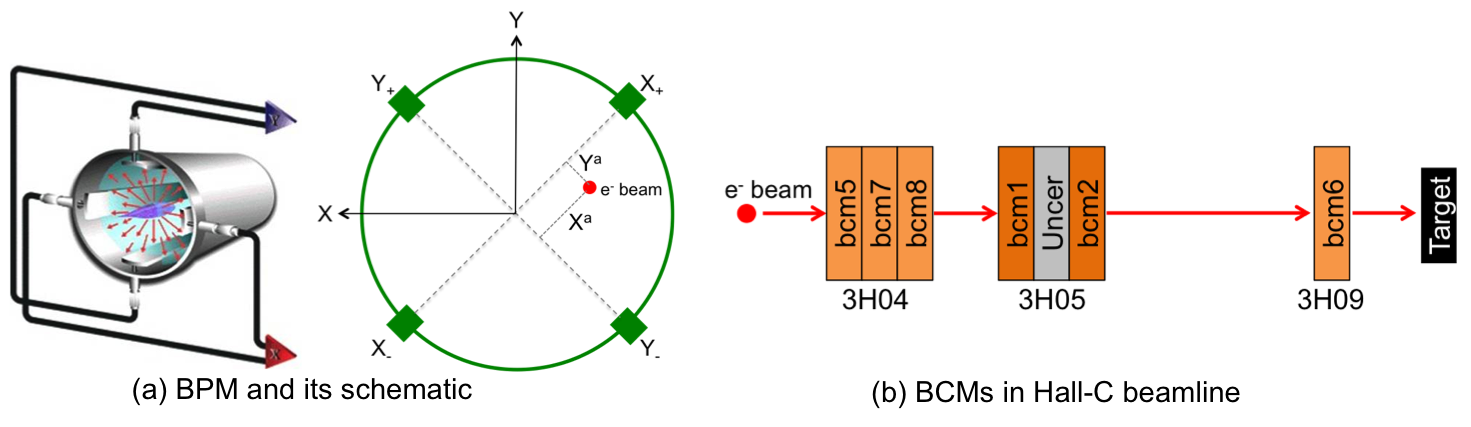
\includegraphics[width=15.0cm]{figures/beam_monitor}
	\end{center}
	\caption
%	[Beam position and current monitors.]
	{Beam position and current monitors. (a) Beam Position Monitors with four antennae rotated by 45$^o$ in the plane. Z axis is perpendicular to the plane. (b) Beam Current Monitors and their locations at Hall-C.}
	\label{fig:beam_monitor}
\end{figure}
\end{singlespace}

\subsection{Beam Position Monitor\index{BPM}}%
\label{Beam Position Monitor}

The beam position was continuously monitored at many places along the Hall-C beamline and throughout the accelerator by SEE beam position monitors (\newnot{symbol:BPM}BPM\index{BPM}) during data collection to ensure that the beam was centered on the target. Each beam position monitor consists of a resonant cavity of a fundamental frequency equal to that of the accelerator and the Hall-C beam. The position of the beam is measured using four antennae rotated by 45$^o$ in the plane (y axis is in direction opposite to gravity, x is horizontal) perpendicular to beam direction (z-axis) shown in Figure~\ref{fig:beam_monitor} (a).
Four antennae inductively pick up the fundamental frequency of the beam as it passes through the BPM. Then radio frequency (\newnot{symbol:RF}RF\index{RF}) signal from each antena (wire) is processed electronically which yields a \newnot{symbol:DC}DC signal proportional to the beam current times the distance between the wire and the beam. DC signals were sent through voltage-to-frequency\index{voltage-to-frequency} converters and recorded with scalers that are read out by Experimental Physics Industrial Control System (\newnot{symbol:EPICS}EPICS\index{EPICS}), the system used by the accelerator and end stations for slow control and monitoring of accelerator and experiment parameters with the rest of the data from the experiment. The beam position $X^a$ and $Y^a$ along the axis of the wires are calculated by a difference over sum of each opposite wire as:

\begin{equation} \label{equ:bpm1}
X^{a} = k \frac{\left(X_{+} - X_{\textrm{offset+}}\right) - \alpha_{X}\left(X_{-} - X_{\textrm{offset-}}\right)}{\left(X_{+} - X_{\textrm{offset+}}\right) + \alpha_{X}\left(X_{-} - X_{\textrm{offset-}}\right)}
\end{equation}

Where $X_{\textrm{offset+(-)}}$ is the offset for the $X_{+(-)}$ wire, $k$ is the sensitivity of the BPM at 1497~MHz and $\alpha_{X}$ is a measure of the possibly different gain between the $X_{+}$ and $X_{-}$ antennae \cite{sarah_G0,bpm1}. The gain difference $\alpha_X$ is defined as

\begin{equation} \label{equ:bpm2}
\alpha_{X} = \frac{X_{+} - X_{\textrm{offset+}}}{X_- - X_{\textrm{offset-}}}
\end{equation}

The center of gravity of the four antenna signals measures relative changes in the offset of the beam from its ideal trajectory. Same approach is used to compute relative beam position $Y^a$. Then the position of the beam in hall co-ordinate system can be written as:

\begin{equation} \label{equ:bpm3}
\left( \begin{array}{c}
X \\
Y \\
\end{array} \right)
=
\frac{1}{\sqrt{2}}
\left( \begin{array}{cc}
1 & -1\\
1 & 1\\
\end{array} \right)
\left[\left( \begin{array}{c}
X^{a} \\
Y^{a} \\
\end{array} \right)
-
\left( \begin{array}{c}
X^{a}_{\textrm{offset}} \\
Y^{a}_{\textrm{offset}} \\
\end{array} \right)\right]
\end{equation}

The information from BPM for a event can not be understood as the exact beam position on target for that event, as the signals are not synchronized with the event data itself and also the actual position on target is constantly changing due to the fast raster system. Practically, an average beam position is calculated using a rolling average of BPM data information over a specified number of previous events depending on the experiment data rate. This average beam position is then corrected for each event using the fast raster signals~\cite{puckett_GEPIII}. Normally average beam position on target is very stable over the period of a single \newnot{symbol:CODA}CODA\index{CODA} run, it is more practical to simply ignore the event-by-event BPM information and fix the average beam position as a parameter of the analysis, and to use the raster signals to measure the change in beam position relative to the fixed average position. BPMs were calibrated using the super harps in Hall-C beamline \cite{hauger_polarimeter}. Typically calibrated BPMs has a resolution of 1~$\mu$m. 
%More details about BPM  resolution will be discussed in analysis chapter. 
Basic details about BPMs can be found in~\cite{bpm2}.

Six BPMs in the Hall-C beamline over a span of 10~m upstream of the target were used to project the beam path at the target continuously during the experiment. Error averaged postion changes over six BPMs were used to measure the position and angle changes at the target, where BPMs in front of the target were used for the same to verify the result. Detail description about the target BPM\index{BPM!target BPM} can be found in~\cite{nur_linear_reg, leo_book} and B. Waidyawansa's thesis~\cite{buddhini_qweak}.


\subsection{Superharp\index{Superharp}}%
\label{Superharp}

A more precise and accurate determination of the beam position and profile is obtained using the superharp system. Each superharp consists of a set of two vertical wires and one horizontal wire strung on a moveable frame. These wires can be scanned across a low current beam to measure its profile and absolute position. The signals induced on the wires as they are scanned across the beam are digitized by an analog to digital converter (\newnot{symbol:ADC}ADC\index{ADC}) and correlated with the wire positions as recorded by an encoder equipped with absolute position readout electronics. Since a harp scan interferes destructively with the electron beam, data taking must be interrupted to perform the measurement. In addition to measuring the beam profile, the superharp system provided a reference coordinate against which the BPMs were calibrated.


\subsection{Beam Current Monitor\index{BCM}}%
\label{Beam Current Monitor}

\v{C}erenkov detector yields were normalized with beam current monitors to remove charge fluctuation . A series of six beam current monitors (\newnot{symbol:BCM}BCMs) were used continuously for relative measurement of the beam current in the Hall-C beamline (as shown in Figure~\ref{fig:beam_monitor} (b)). The BCMs were coupled cylindrical stainless steel resonant cavities~\cite{bclasie,nur_kaon_thesis} whcih were used to measure the beam current by measuring resonance of the TM$_{010}$ mode at 1497~MHz. This signal then converted to a voltage in a RMS-DC voltage converter and read by TRIUMF made \newnot{symbol:ADC}ADCs. This voltage signal also sent to a 1~MHz voltage to frequency (V-F) converter and scalers for event-mode normalization. 
In the beginning only available BCMs were 1 and 2 and latter BCMs 5, 6, 7, 8 with low noise digital receiver were added. 
BCMs were calibrated using a parametric current transformer device called Unser\index{BCM!Uncer} monitor for the high beam current (1-180~$\mu$A) where as for low current (10~nA to 1~$\mu$A) a Faraday cup was used for calibration.
The detector yields were normalized with BCM1 and 2 during Run-I and BCM8 during Run-II. Nominal current measured by these BCMs during production running was 180~$\mu$A. More details about BCMs used during the Q-weak experiment is discussed in a technical report by Ramesh Subedi~\cite{ramesh_bcm}.


\subsection{Beam Energy\index{Beam Energy}}%
\label{Beam Energy}

The four momentum transfer squared, $Q^{2}$ is approximately proportional to square of absolute energy, $E^{2}$ (see Equation~\ref{equ:kinQ2}), and measured precisely. Energy asymmetry was also measured to remove false asymmetry. 

\subsubsection{Absolute Beam Energy\index{Absolute Beam Energy}}%
\label{Absolute Beam Energy}

The Hall-C beamline arc was used as a spectrometer to measure the absolute beam energy~\cite{Yan:1993fd}. The initial beam energy before scattering was defined as the absolute beam energy. 
%An electron passes through an arc changes its momentum and can be expressed as 
An electron passing through magnetic fields, such as the beamline arc, changes its direction. That change can be related to the momentum as

\begin{equation} \label{equ:energy1}
p = \frac{e}{\Delta\theta} \int Bdl
\end{equation}

\noindent
where $\Delta\theta$ is the change in bending angle through the arc and $\int Bdl$ is the magnetic field integral over the electron path. Three set of superharp scanners~\cite{Yan1995261} were used to determine the position and the angle by scanning the beam at the beginning, end, and middle of the Hall-C (or 3C\footnote{According to JLab accelerator division coordinate system, 3C symbolize for Hall-C beamline. Similarly 1C and 2C represents Hall-A and Hall-B beamlines, respectively.}) arc. All the active elements (quadrupole, corrector magnets) of the beamline were turned off to avoid any distortion. This procedure is an invasive process and needed dedicated measurements. A typical energy measurement using this method yield energy as 1160.39 $\pm$ 1.74~MeV~\cite{kmyers_qweak}. 


\subsubsection{Energy Asymmetry\index{Energy Asymmetry}}%
\label{Energy Asymmetry}

One of the helicity correlated beam parameter is beam energy asymmetry. Small 
%changes in the energy asymmetry 
deviations of the energy asymmetry from zero 
could result into false asymmetry, hence precise measurement of the energy asymmetry was important for Q-weak. In the middle of the 3C arc has the highest dispersion and is represented as 3C12 in JLab accelerator coordinate system. Any change in beam energy could result a big horizontal position change in the 3C12. Then relative energy change at the target can be expressed as

\begin{equation} \label{equ:energy2}
\Delta\left(\frac{dE}{E} \right)_{\textrm{target}} = \frac{1}{M_{15}}\Delta X_{\textrm{3C12}} - \frac{M_{11}}{M_{15}}\Delta X_{\textrm{target}} - \frac{M_{12}}{M_{15}}\Delta X^{\prime}_{\textrm{target}}
\end{equation}

\noindent
where $\Delta X_{\textrm{3C12}}$, $\Delta X_{\textrm{target}}$, $\Delta X^{\prime}_{\textrm{target}}$ are position change at 3C12, position change at target, and angle change at the target, respectively. First order beam transport matrix between 3C12 and target $M_{11}$, $M_{12}$, and $M_{15}$ were determined using OptiM~\cite{OPTIM}. This calculation works for linear models and any residual dispersion at the target or X-Y coupling are not considered in this first order calculation. More details about this model will be discussed in the following chapter. Typical energy asymmetry at the target during the experiment was $\mathcal{O}$(1)~ppb. 

\subsection{Beam Modulation\index{Beam Modulation}}%
\label{Beam Modulation Experiment}

The e-p scattering rate in first order depends on five beam parameters: horizontal position ($X$), angle ($X^\prime$), vertical position ($Y$), angle ($Y^\prime$), and beam energy ($E$). Changes in these beam parameters when the beam polarization is reversed can create false asymmetries. Although different techniques were used to keep helicity-correlated parameter changes as small as possible, must need to correct for such false asymmetries. To do this, $X$, $X^{\prime}$, $Y$, $Y^{\prime}$ were modulated using four air-core dipoles in the Hall C beamline and beam energy was modulated using a superconducting RF cavity. The goal of the beam modulation system was to occasionally induce controlled beam parameter changes $\Delta X_{i}$, measure the resulting detector false asymmetry\index{False Asymmetry} $A_{\textrm{false}}$, and determine the detector sensitivities $\partial A$/$\partial X_{i}$. This will allow later correction of beam false asymmetries via 

\begin{equation} \label{equ:bm1}
A_{\textrm{false}} = \sum^{5}_{i=1}\frac{ \partial A }{ \partial X_{i} } \Delta X_{i}.
\end{equation}

Even if these corrections prove to be small under ideal running conditions, the modulation system will allow the determination of any undesirable changes~\cite{nur_bm_final}. 
A dedicated chapter on beam modulation system will be discussed in following chapter.



\subsection{Halo Monitors\index{Halo Monitors}}%
\label{Halo Monitors}

Another important property of the beam is the beam halo which refers to stray electrons that move along with the primary beam but are sufficiently far from the beam center and can contribute in the background. Beam halo can be generated via space-charge effects from of electrons during bunching, scraping in the beam pipe, or poor vacuum and can be measured using plastic Lucite detector and scintillation counters. 
%Apertures on the halo target were 8 mm square opening and 13 mm diameter hole. 
An 8~mm square opening and 13~mm diameter hole were used as halo targets. The halo monitors were located immediately downstream of the halo targets and upstream of the LH$_{2}$ target. The beam halo can also be estimated using the main detectors and luminosity monitors which can be normalized using the hole targets.


\subsection{Fast Feed Back\index{Fast Feed Back}}%
\label{Fast Feed Back}

The electron beam at JLab is troubled by the fluctuation in beam position and energy. These fluctuations mostly occur at the power line frequencies of 60, 120, 180 etc.~Hz and rooted in the electromagnetic fields generated by the accelerator electronic equipment~\cite{jlab_ffb1}. These deviations were largely nullified using Fast Feed Back (FFB) system by applying real time corrections targeted at the power line harmonics~\cite{jlab_ffb2} to the RF verniers along the beamline. The FFB system was implemented by modifying the existing BPM system and integrating it to the algorithm for correction signals. The control system for FFB is EPICS based which provides a graphic interface on Unix workstations connected via Local Area Network (LAN) to a Input/Out Controller (IOC\footnote{VME bus embedded processor}). The FFB system was able to correct the energy fluctuation better than 10$^{-4}$ at power line harmonics up to 720~Hz using a frame rate of 3~kHz~\cite{jlab_ffb1}.

%%%%%%%%%%%%%%%%%%%%%%%%%%%%%%%%%%%%%%%%%%%%%%%%%%%%%%%%%%%%%%%%%%%%%%%
\section{Polarimetry\index{Polarimetry}}%
\label{Polarimetry}

One of the dominant systematic experimental uncertainties for the Q-weak experiment come from 
%The most dominant systematic experimental uncertainty for the Q-weak experiment is expected to come from 
a 1\% absolute uncertainty on beam polarization as shown in Table~\ref{tab:qweak_proposal}. In order to achieve this goal two polarimeters, a well tested invasive low current M{\o}ller polarimeter and noninvasive relatively new Compton polarimeter, were used to measure the beam polarization.

\begin{singlespace}
\begin{figure}[!h]
	\begin{center}
	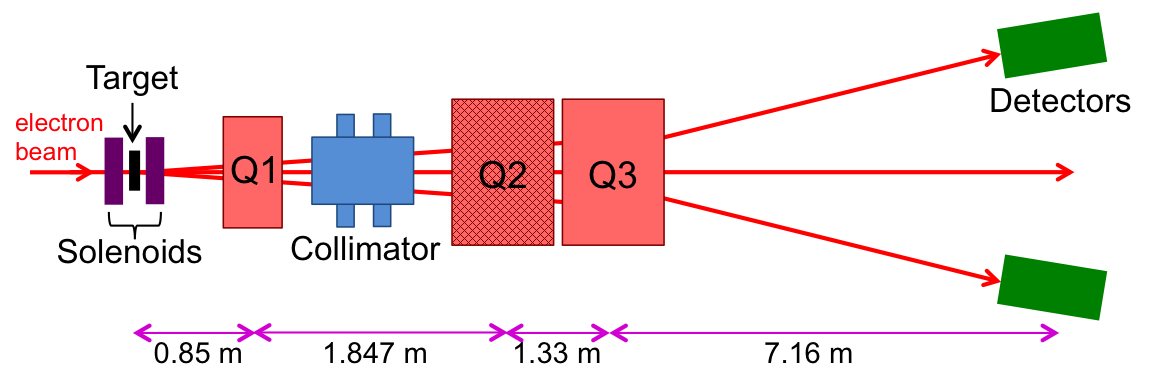
\includegraphics[width=15cm]{figures/moller}
	\caption
%	[Layout of the Hall C M{\o}ller polarimeter.]
	{Layout of the Hall C M{\o}ller polarimeter showing tin foil target, set of superconducting solenoids, quadrupoles (Q2 was off during Q-weak), collimator box, and symmetric detectors.}
	\label{fig:moller}
	\end{center}
\end{figure}
\end{singlespace}

%\subsection{M{\small$\varnothing$}ller Polarimetry\index{Polarimetry!Moller}}%
\subsection{M{\o}ller Polarimetry\index{Polarimetry!M{\o}ller}}%
\label{Moller Polarimetry}
The M{\o}ller polarimeter is used to measure the polarization of the longitudinally polarized electron beam entering Hall-C \cite{Hauger2001382}. To accomplish this goal, the polarimeter measures the spin-dependent asymmetry in the elastic scattering of polarized electrons from polarized electrons i.e. e$^{-}$ + e$^{-}$ $\rightarrow$ e$^{-}$ + e$^{-}$(M{\o}ller scattering). This is a pure Quantum Electrodynamics (\newnot{symbol:QED}QED) process and its cross section can be calculated accurately. The target used for the scattering is a thin foil of iron magnetized by superconducting solenoids with field of $\sim$4~T. A set of quadrupole magnets Q1 and Q3 were used (Q2 was off during the experiment) 
%\footnote{some beamline optics survey suggested leakage current in Q2  and will be discussed in details in latter chapter} 
to focus the scattered and recoiled electrons in to the symmetric detectors in coincidence. Then detectors measure the asymmetry and then compute the polarization after correcting for the backgrounds. Figure~\ref{fig:moller} shows the layout of the Hall-C Basel M{\o}ller polarimeter. It was designed to operate with currents lower than 8~$\mu$A whereas Q-weak production current was 180~$\mu$A. During the experiment, M{\o}ller measurements were performed invasively at low currents (1~$\mu$A) three times a week. The typical measured longitudinal polarization using the M{\o}ller polarimeter was about 88\%. A sample of the M{\o}ller result will be shown in later chapters. More elaborated description of the M{\o}ller polarimeter can be found in M. Loppacher's thesis~\cite{Loppacher_moeller_thesis} and polarization technique used during Q-weak can be found in R. Beminiwattha's~\cite{rakitha_qweak} thesis.

\begin{singlespace}
\begin{figure}[!h]
	\begin{center}
	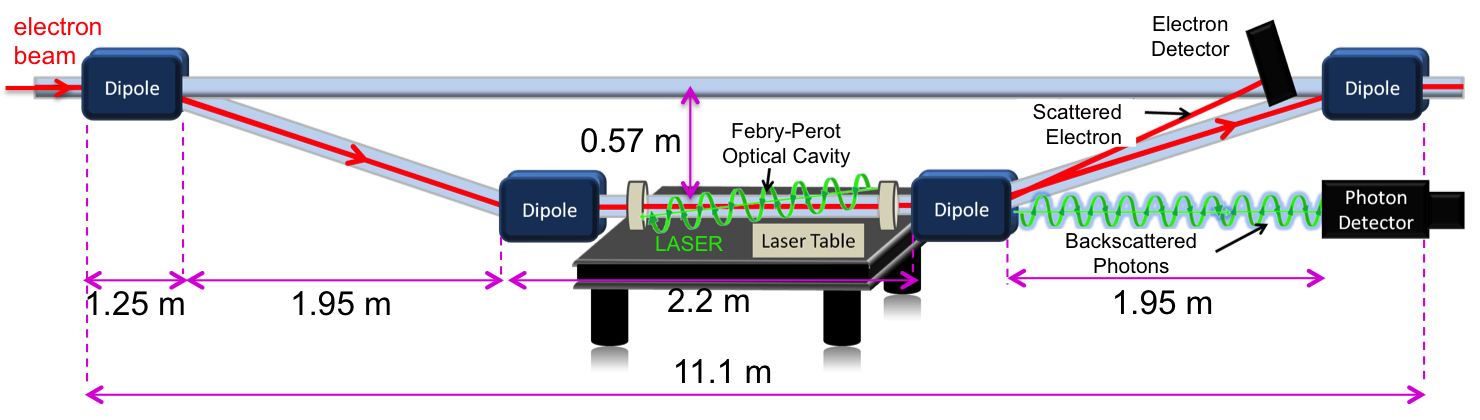
\includegraphics[width=15cm]{figures/compton}
	\caption
%	[Schematic of the Hall C Compton polarimeter.]
	{Schematic of the Hall-C Compton polarimeter. The incoming electron beam interacts with the green LASER at the straight section of the chicane. The scattered electrons and back-scattered photons are detected by electron detector and photon detector, respectively for each helicity (MPS) state.}
	\label{fig:compton}
	\end{center}
\end{figure}
\end{singlespace}

\subsection{Compton Polarimetry\index{Polarimetry!Compton}}%
\label{Compton Polarimetry}

A new Hall-C Compton polarimeter was installed and used for the Q-weak experiment~\cite{presentation:amar_compton_1732}. This was a noninvasive high current polarimeter and continuously took data during production data taking ( with $\sim$180~$\mu$A). The apparatus for the Compton polarimeter includes four dipoles in a chicane, a green \newnot{symbol:laser}laser, an electron detector, and a photon detector as shown in Figure~\ref{fig:compton}. The Compton polarimeter use the Compton scattering (e$^{-}$ + $\gamma$ $\rightarrow$ e$^{-}$ + $\gamma$) of the incident electron beam with photons from a green laser. The scattered electrons and back-scattered photons provides two independent measurement of the polarization using  both electron and photon detector, respectively. The dipole chicane were used to move the interaction point away from primary beam in order to detect back-scattered photons in the photon detector. A CsI crystal with photo multiplier tube was used as photon detector. Later in the experiment germanium silicon oxide (GSO), and led-tungstate (PbWO$_{4}$) were used instead of CsI in the photon detector. The electron detector consist of radiation hard diamond micro-strips and for the first time used as a tracking device in an experiment. The scattered electrons were detected in a array of 96 diamond strips after third dipole. There were four detector planes, each with 200~$\mu$m thick 96 strips, and were readout by four VME 1495 boards. The measured beam polarization using Compton polarimeter was about 87-89\%. A sample of Compton result will be shown in later chapters. More detailed description of Compton polarimeter and its electron and photon detector measurements will be discussed by A. Narayan ~\cite{amar_compton_thesis} and J. Cornejo~\cite{carlos_compton_thesis}, respectively in their future theses.


%%%%%%%%%%%%%%%%%%%%%%%%%%%%%%%%%%%%%%%%%%%%%%%%%%%%%%%%%%%%%%%%%%%%%%%
\section{Targets\index{Targets}}%
\label{Targets}

The Q-weak target system has two main components: a main liquid hydrogen (\newnot{symbol:LH$_{2}$}LH$_{2}$) cell for production data taking and a matrix of solid targets used for background measurements and ancillary tests. Solid target ladder was thermally coupled to the bottom of the LH$_{2}$ cell. A schematic of the target system is shown in Figure~\ref{fig:target}.


\begin{singlespace}
\begin{figure}[!h]
	\begin{center}
	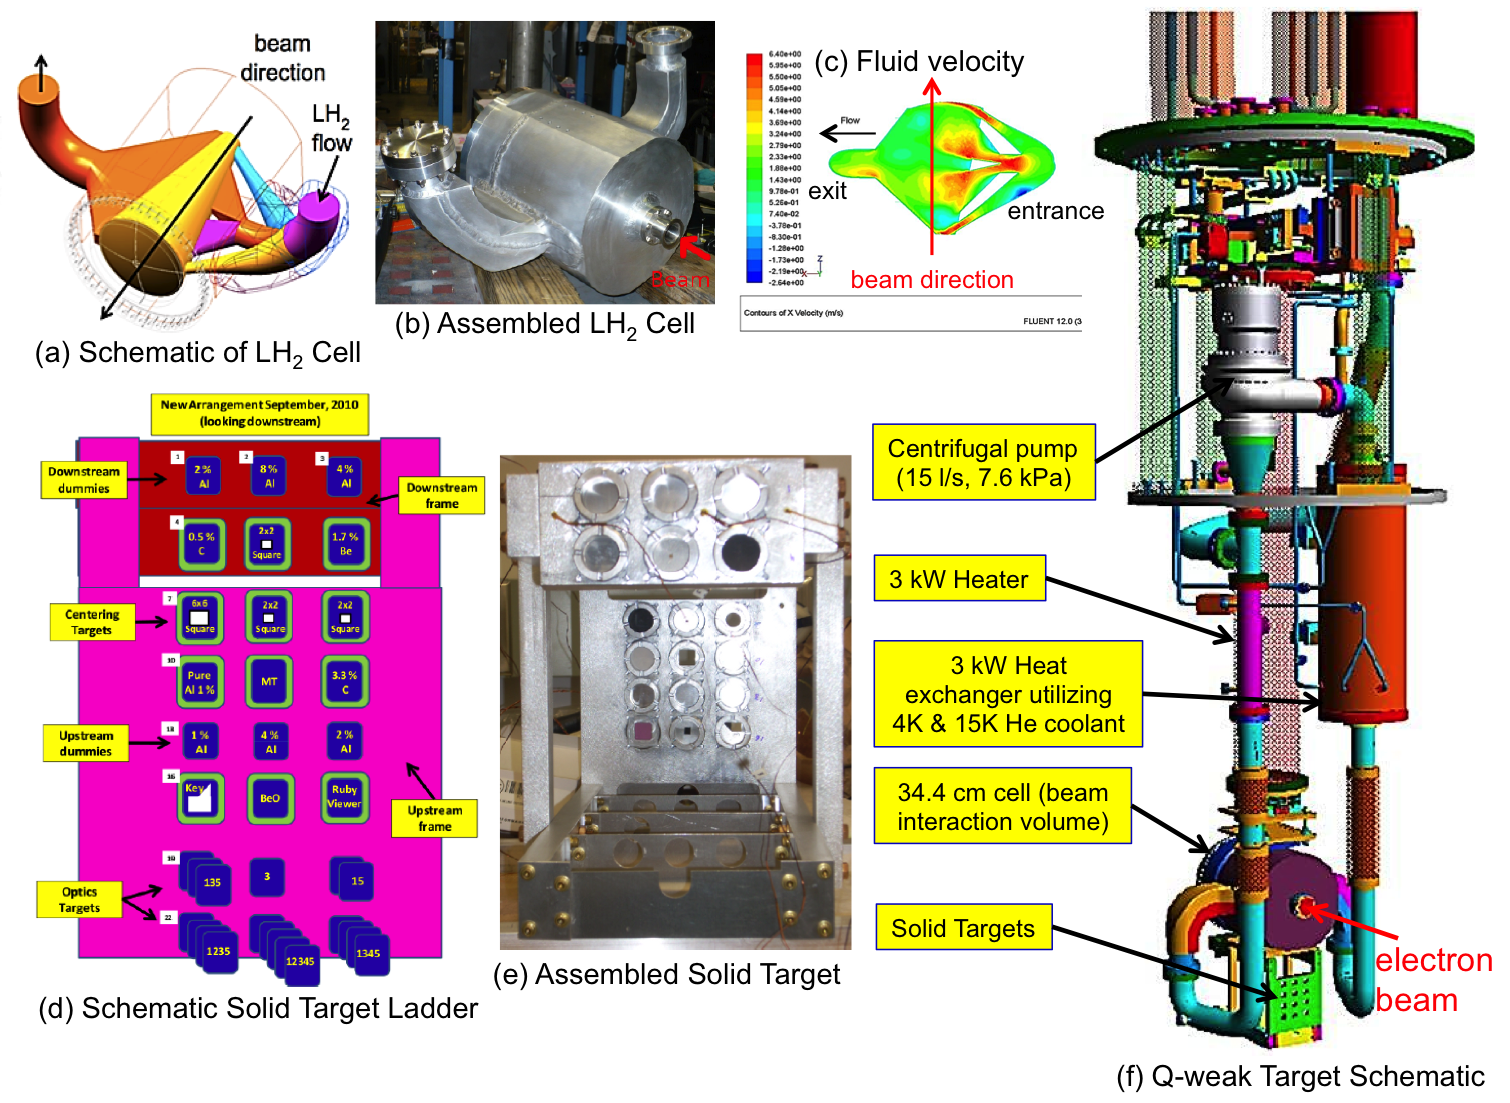
\includegraphics[width=15cm]{figures/target}
	\caption
%	[Q-weak target system.]
	{Q-weak target system. (a) Canonical shaped Computer Aided Drawing (\newnot{symbol:CAD}CAD) model of target cell design. (b) Assembled LH$_{2}$ target cell. (c) Simulation of LH$_{2}$ velocity contours inside target cell using \newnot{symbol:CFD}CFD. (d) Schematic of solid target ladder. (e) Assembled solid target. (f) Full schematic of the target system with key components like main LH$_{2}$ target cell, pump, heater, heat exchanger, solid targets are shown. }
	\label{fig:target}
	\end{center}
\end{figure}
\end{singlespace}
%


\subsection{Liquid Hydrogen Target\index{Targets!Liquid Hydrogen Target}}%
\label{Liquid Hydrogen Target}

A 34.4~cm long liquid hydrogen (\newnot{symbol:LH$_{2}$}LH$_{2}$) cell was used as the primary target for the Q-weak experiment \cite{greg_target_hydrogen}. This target can dissipate 2.5~kW of power deposited by the 1.155~GeV, 180~$\mu$A, 4~mm $\times$ 4~mm rastered 
%(more details in section~\ref{Raster}) 
electron beam and is the highest powered cryogenic target in the world to date. A unique hybrid cooling system used at JLab is End Station Refrigerator (\newnot{symbol:ESR}ESR) for 15~\newnot{symbol:K}K coolant and the Central Helium Liquefier (\newnot{symbol:CHL}CHL) for 4 K coolant were mixed at the heat exchanger (Figure~\ref{fig:target} (f)). A high power heater was used to replace the heat deposited by the electron beam in case of beam trips. It also helped to stabilize the LH$_{2}$ target temperature in conjunction with 15 K and 4 K coolant in a proportional integral derivative (\newnot{symbol:PID}PID) feedback system. The 55~liters of LH$_{2}$ was contained within a target cell of thin aluminum (Al) alloy window and was operated under 35 psi pressure at 20~K temperature and with a transverse flow of 1.2~\newnot{symbol:kg}kg/\newnot{symbol:s}s maintained by modified automobile centrifugal turbo pump at frequency of 30~Hz. 

This long canonical shaped (see Figure~\ref{fig:target} (a,b)) cell accommodated required 7.9\degrees{} scattering angle and helped to achieve the high luminosity and hence the statistical goal. The current mode production data taking was very sensitive to target density fluctuation as such, the target was designed using Computational Fluid Dynamics (\newnot{symbol:CFD}CFD) and simulated using ANSYS \cite{website:ansys} (a fluid dynamics simulation code) to minimize noise from density fluctuations and maintain nominal fluid density. The simulation shows the main hot spots were entrance and exit windows of the cell as shown in Figure~\ref{fig:target} (c). The exit window was 0.02~inch thick aluminum alloy with a 10 inch radius of curvature and a 0.005~inch nipple to minimize backgrounds.


\begin{singlespace}
\begin{figure}[!h]
	\begin{center}
	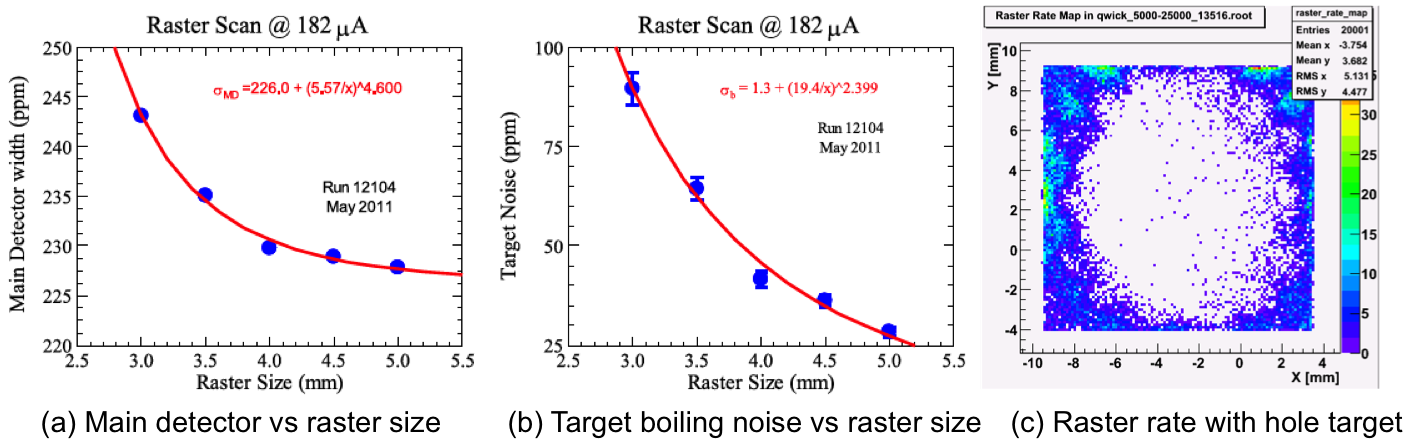
\includegraphics[width=15cm]{figures/raster}
	\caption
%	[Raster studies.]
	{Raster studies. (a) Main detector width dependence on raster. (b) Target boiling noise studies at 180~$\mu$A\cite{kmyers_qweak}. (c) 2d raster rate map with a hole target.}
	\label{fig:raster}
	\end{center}
\end{figure}
\end{singlespace}

\subsubsection{Raster\index{Raster}}%
\label{Raster}

The intrinsic size of the electron beam (perpendicular to beam direction) at JLab is $\sim$2~$\mu$m and creates localized high power density on the LH$_{2}$ target. This could result in boiling the target. Hence the beam was rastered on the target over an area of 4~mm $\times$ 4~mm by the fast raster\index{Raster!Fast Raster} system.
The raster was designed to have a matching beat frequency with fast helicity flip of 960~Hz. This method assures each integration period has the same complete raster pattern on the target and prevents systematic differences in the beam position between Macro Pulse Signal (\newnot{symbol:MPS}MPS). The contribution of target density fluctuation and raster size dependence to the statistical width was measured by using known detector asymmetry widths from statistics and other sources (shown in Figure~\ref{fig:raster} (a)). In typical production running with 180~$\mu$A, 4~mm $\times$ 4~mm rastered beam the contribution from target boiling noise was 46~ppm (shown in Figure~\ref{fig:raster} (b)), which is relatively small contribution to the statistical width of $\sim$200~ppm.

\subsection{Solid Target\index{Targets!Solid Target}}%
\label{Solid Target}

Along with LH$_{2}$ target an array of solid targets \cite{greg_target_solid} consist of aluminum (\newnot{symbol:Al}Al) dummy targets, optics targets, and centering targets were used for background and ancillary measurements. The solid target ladder was thermally coupled to the bottom of the LH$_{2}$ cell as shown in Figure~\ref{fig:target} (f). A detailed schematic of solid target matrix looking upstream is shown in Figure~\ref{fig:target} (d,e). Horizontal and vertical motion controller were used to insert different targets into the beam. Three different Al dummy target thicknesses for both upstream and downstream locations were used to measure the effect of radiative corrections in the measured asymmetry. The optics targets were primarily used for particle origin reconstruction in the tracking measurements. Optics target helped to locate the position of the target ladder in raster rate scan as shown in Figure~\ref{fig:raster} (c). 

%\begin{singlespace}
%\begin{figure}[!h]
%	\begin{center}
%	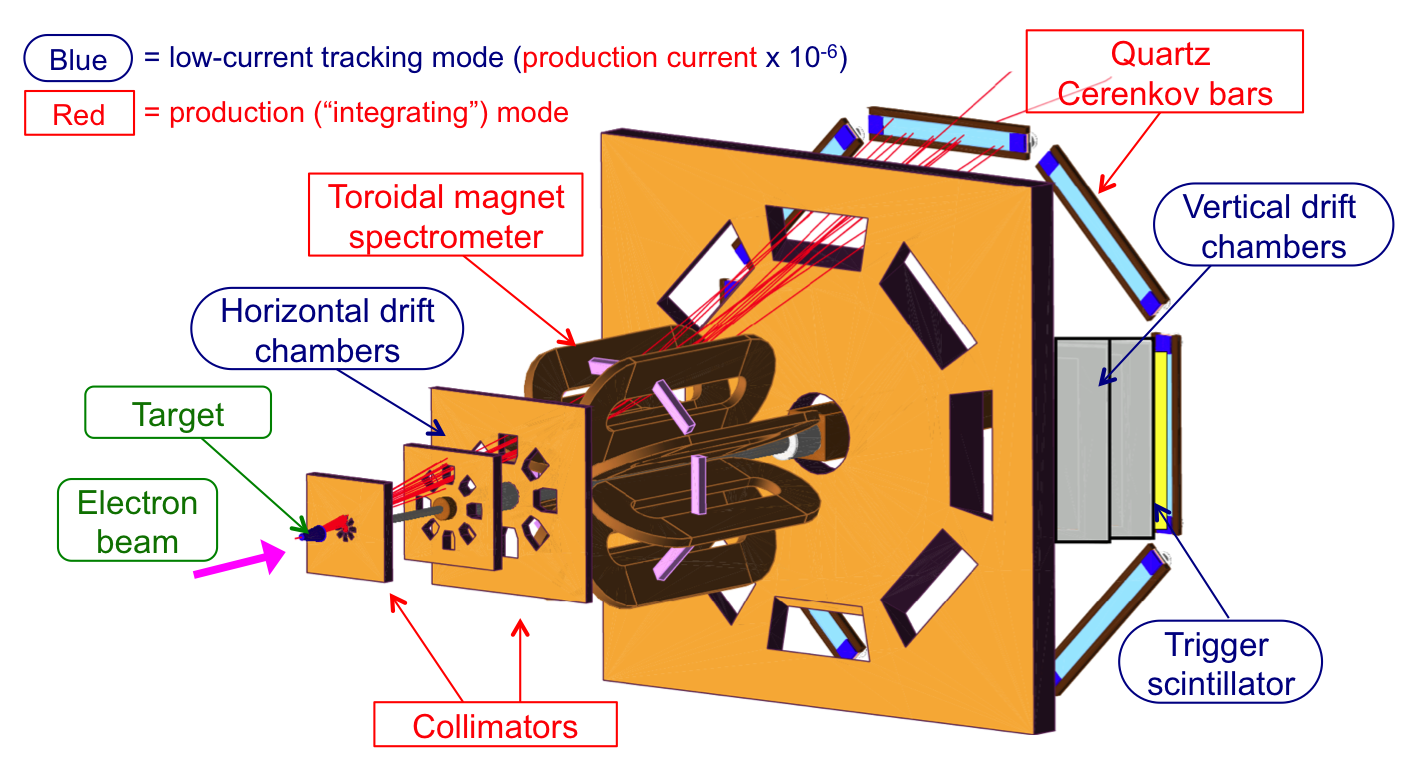
\includegraphics[width=15.0cm]{figures/qweakApparatus}
%	\end{center}
%	\caption[Schematic diagram of the Q-weak apparatus.]{Schematic diagram of the Q-weak apparatus. The basic experimental design showing the target, collimators, toroidal magnet coils, electron trajectories, and detectors. Elastically scattered electrons focus at the \v{C}erenkov detectors. High current production mode apparatus components are shown in red rectangular boxes and low current tracking mode components are shown in blue elliptical boxes. Beam direction is from left to right.}
%	\label{fig:qweakApparatus}
%\end{figure}
%\end{singlespace}

\begin{singlespace}
\begin{figure}[!h]
	\begin{center}
	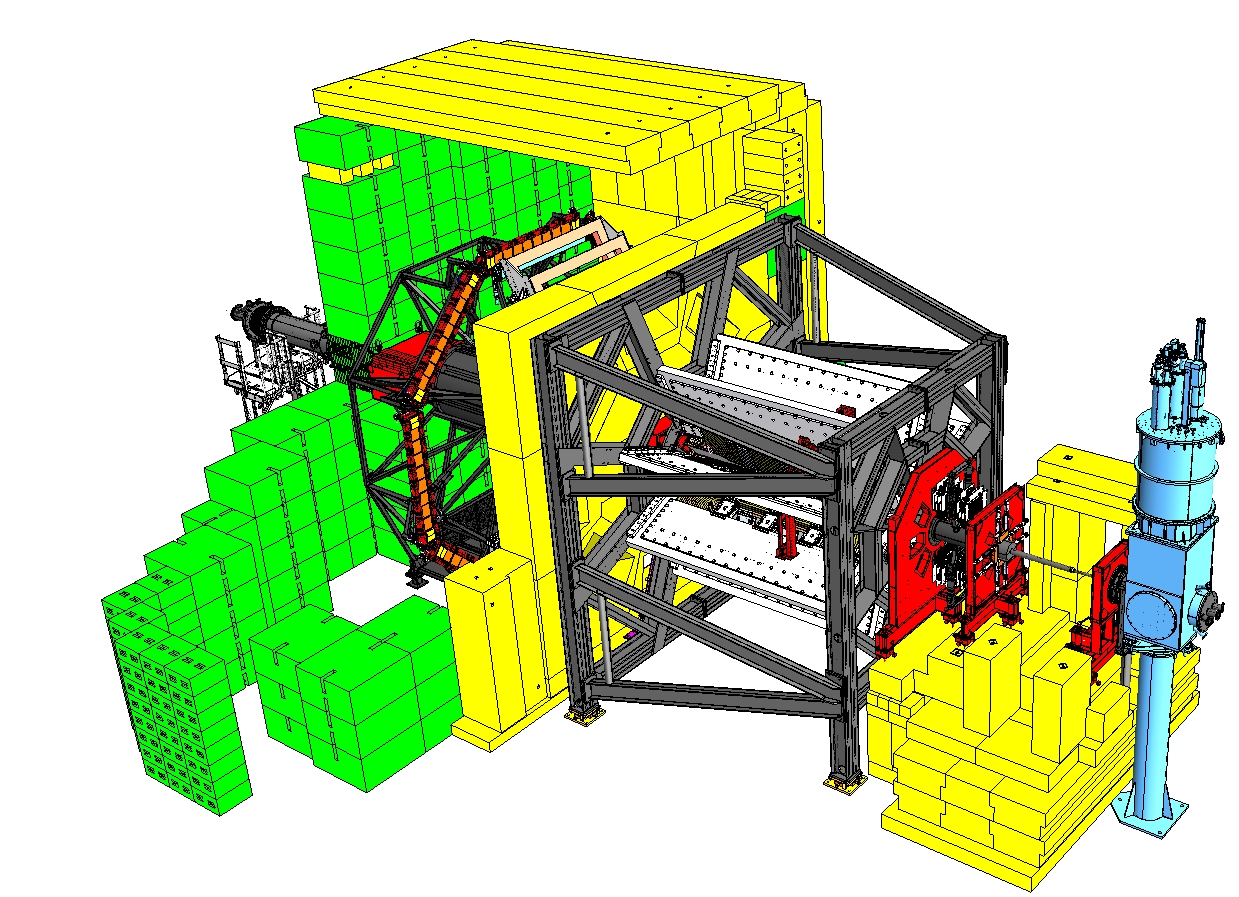
\includegraphics[width=15.0cm]{figures/Q-weak_Appratus}
	\end{center}
	\caption
%	[Schematic diagram of the Q-weak apparatus.]
	{Schematic diagram of the Q-weak apparatus. The basic experimental design showing the target, collimators, toroidal magnet coils, and detectors. Elastically scattered electrons focus at the \v{C}erenkov detectors. High current production mode apparatus components are shown in red rectangular boxes and low current tracking mode components are shown in blue elliptical boxes. Beam direction is from right to left.}
	\label{fig:qweakApparatus}
\end{figure}
\end{singlespace}
	
%%%%%%%%%%%%%%%%%%%%%%%%%%%%%%%%%%%%%%%%%%%%%%%%%%%%%%%%%%%%%%%%%%%%%%%
\section{Collimators and Shielding\index{Collimator} \index{Shielding}}%
\label{Collimator and Shielding}

A set of three lead collimators were used to define the experiment's angular acceptance and minimize the inelastic and neutral background contribution to the detector. The collimator system is shown in Figures~\ref{fig:qweakApparatus} and~\ref{fig:QTor} (c). The first collimator, a water cooled tungsten plug of inner radius $\sim$7~mm, was placed just downstream of the target and was used to reduce the electron scattering from the beamline. The second (or primary) collimator defined the acceptance as 4\% of $\pi$ in $\theta$ and  49\% of 2$\pi$ in $\phi$. The angular acceptance of the primary collimator from the upstream end of the target window is $\theta$ = 5.8\degrees{} - 10.2\degrees{} and $\theta$ = 6.6\degrees{} - 11.5\degrees{} from the downstream end. The third collimator was before the Q-weak Toroidal Magnetic Spectrometer (QTor) and further cleaned the electron flux before it reached to QTor magnetic field. Besides these three collimators a 80~\newnot{symbol:cm}cm thick shielding wall of barite-loaded (Ba$_{2}$SO$_{4}$) high-density (2.7~g/cm$^{3}$) concrete was used after QTor for addition shielding. A details description of shield wall and collimator system can be found in J. Mammei~\cite{juliette_G0_thesis}, and K. Myers's~\cite{kmyers_qweak} theses.

\begin{singlespace}
\begin{figure}[!h]
	\begin{center}
	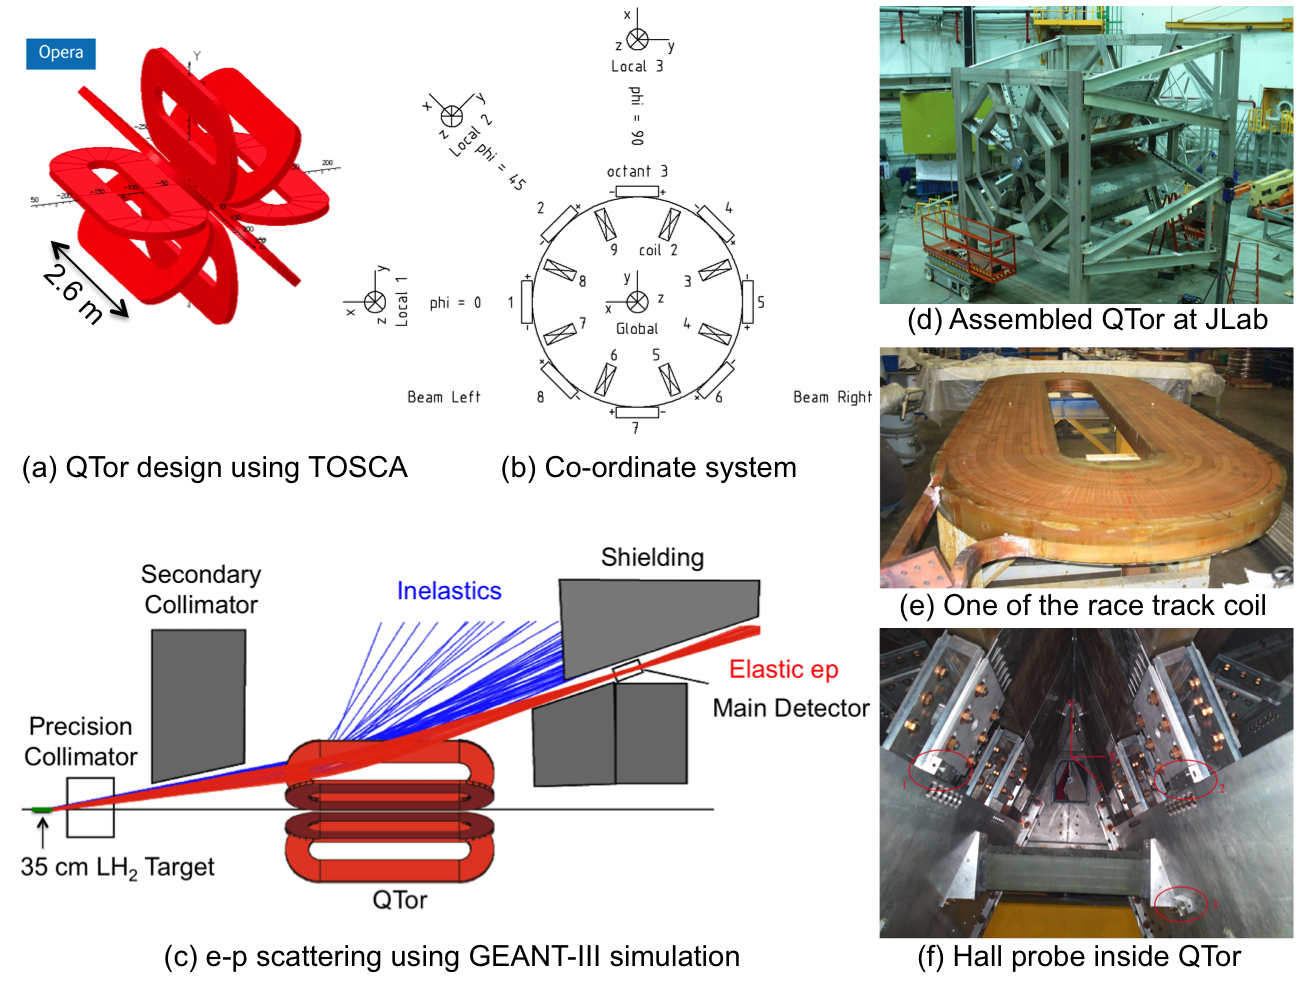
\includegraphics[width=15cm]{figures/QTor}
	\caption
%	[Q-weak torodial magnetic spectrometer (QTor).]
	{Q-weak torodial magnetic spectrometer (QTor). (a) QTor design using TOSCA. (b) Co-ordinate system. (c) e-p scattering using GEANT-III simulation. (d) Assembled QTor at JLab. (e) One of the race track coil. (f) Hall probe inside QTor. }
	\label{fig:QTor}
	\end{center}
\end{figure}
\end{singlespace}



%%%%%%%%%%%%%%%%%%%%%%%%%%%%%%%%%%%%%%%%%%%%%%%%%%%%%%%%%%%%%%%%%%%%%%%
\section{Q-weak Toroidal Magnetic Spectrometer: QTor\index{QTor}}%
\label{QTor}

The eight fold symmetric torodial magnetic spectrometer used for the Q-weak experiment is known as QTor (shown in Figure~\ref{fig:QTor} (a,d)). It has race track shaped water cooled copper (iron free) magnetic coils (shown in Figure~\ref{fig:QTor} (e)). The dimensions of the each magnet coil are 2.2~m long along the straight section, 0.235~m of inner radius, and 0.75~m of outer radius. Eight such identical coil packages with $\Delta\phi$ $\sim$ 45\degrees{} gaps between them made the QTor structure (relevant coordinate system is shown in Figure~\ref{fig:QTor} (b)). The primary objective of QTor magnet was to focus the elastically scattered electron to the main \v{C}erenkov detector in the focal plane of the asymmetry measurement (shown in Figure~\ref{fig:QTor} (c)). 
Neutral particles (neutrons, photons, etc.) remain unchanged. Also QTor did not affect the unscattered beam as there was no field in the geometric center of the magnet.
During nominal elastic asymmetry measurement QTor was operated at 8921~A whereas during inelastic ($N\rightarrow\Delta$) asymmetry measurement the operational current was 6700~A. The magnet required a 10~kA power supply at 130~V and produced a field integral $\int \vec{B} \cdot \vec{dl}$ = 0.67~\newnot{symbol:T}T.\newnot{symbol:m}m along the central trajectory. P. Wang has more details about the QTor design structure and field map in his master's thesis~\cite{peiqing_qweak_masters}.


\begin{singlespace}
\begin{figure}[!h]
	\begin{center}
	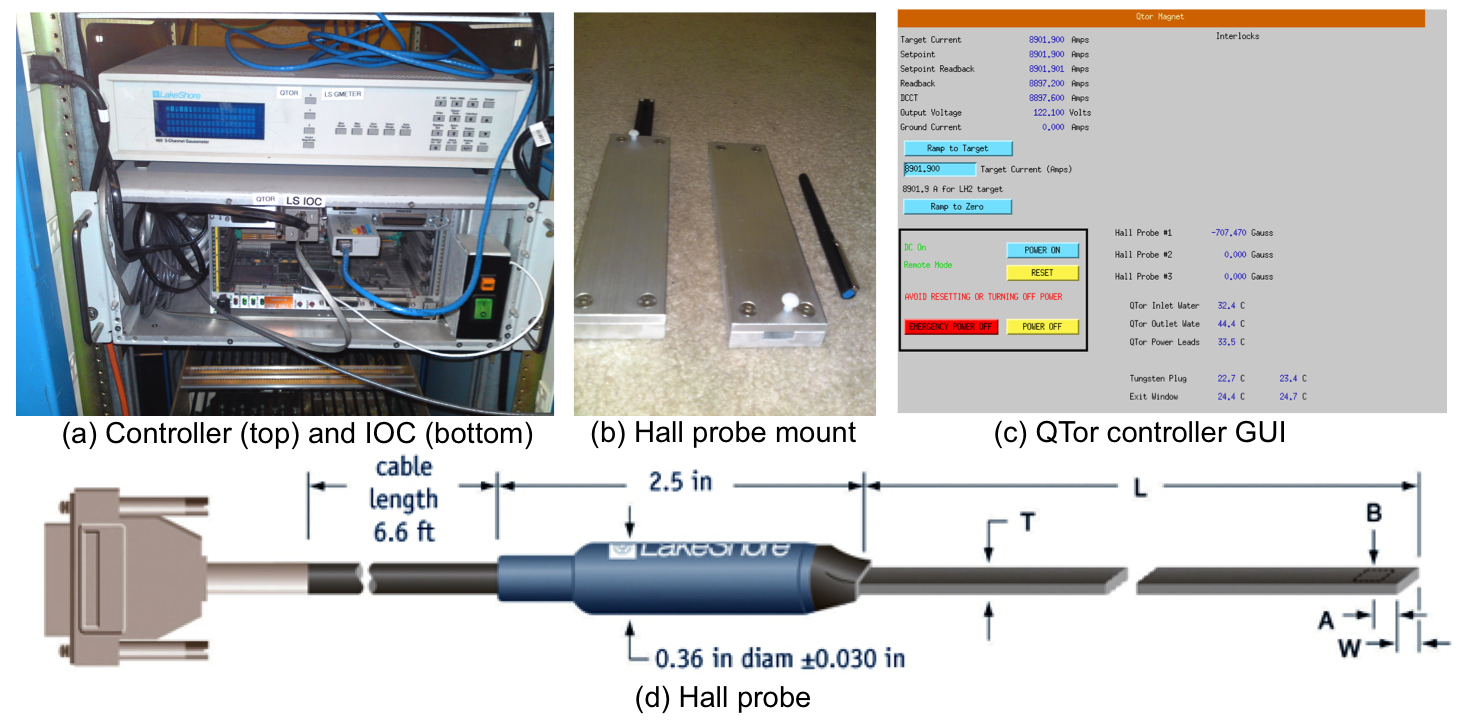
\includegraphics[width=15cm]{figures/QTorHallProbe}
	\caption
%	[QTor controls and hall probe.]
	{QTor controls and hall probe. (a) Lakeshore controller and IOC. (b) Hall probe mount. (c) QTor controller GUI. (d) Hall probe. }
	\label{fig:QTorHallProbe}
	\end{center}
\end{figure}
\end{singlespace}

\subsection{Hall Probe\index{QTOR!hall probe}}
\label{Hall Probe}

A transverse (LakShore MNT-4E02-VH) hall probe was used to measure the QTor magnetic field in real time. Three hall probe mount panels were designed and attached to the inside wall of QTor as shown in Figure~\ref{fig:QTor}(f). The probe was inserted inside the mount and attached with a LakeShore 460 3-channel Gaussmeter controller~\cite{manual_hall_probe} via a 30~m long special magnetically shielded cable (MPEC-100). A VME IOC was then connected with the controller in order to control the system remotely via a CPU (vmec18). EPICS controls were used as a live read back system via the active EPICS channel (Q1HallP). More details about design and functionality of QTor hall probe can be found in~\cite{nur_qtor_hallprobe}.


%%%%%%%%%%%%%%%%%%%%%%%%%%%%%%%%%%%%%%%%%%%%%%%%%%%%%%%%%%%%%%%%%%%%%%%
\section{Detector System\index{Detector System}}%
\label{Detector System}

The Q-weak detector system consists of main \v{C}erenkov detectors and two set of luminosity monitors.  

\begin{singlespace}
\begin{figure}[!h]
	\begin{center}
	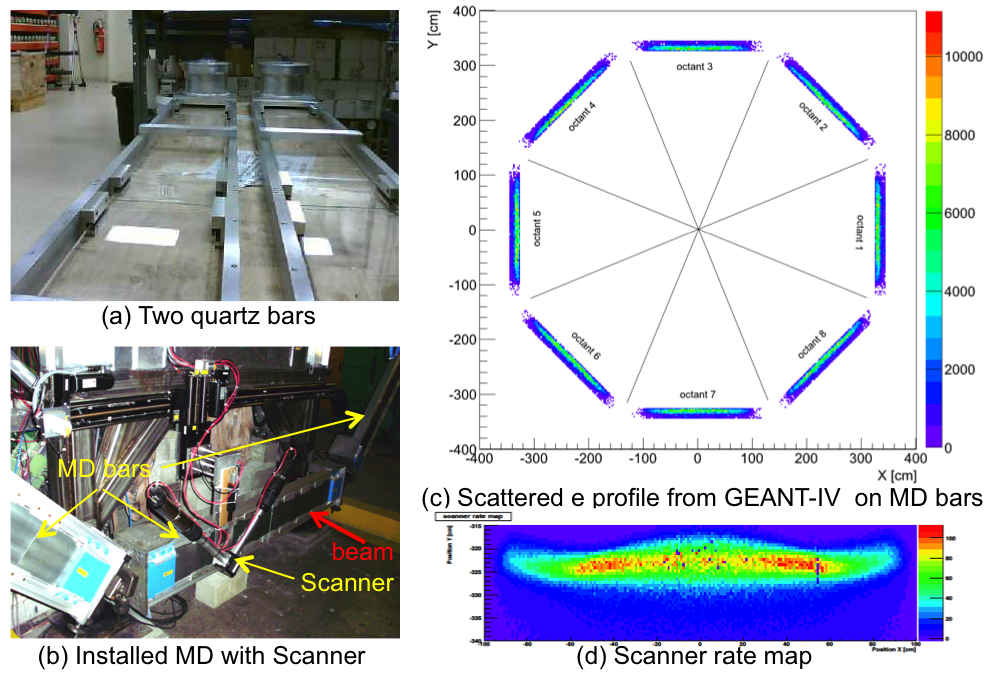
\includegraphics[width=15cm]{figures/main_detector}
	\caption
%	[Q-weak main \v{C}erenkov detector system.]
	{Q-weak main \v{C}erenkov detector system. (a) Two quartz bars. (b) Installed main detectors at Hall-C with scanner system. (c) A GEANT-IV simulation showing elastic scattered electron profile on the quartz bars~\cite{elog:peiqing_analysis588}. (d) The measured rate distribution in MD at 50~$\mu$A beam current with LH$_{2}$ target using scanner~\cite{jie_qweak_thesis}. }
	\label{fig:main_detector}
	\end{center}
\end{figure}
\end{singlespace}

\subsection{Main \v{C}erenkov Detectors\index{Main \v{C}erenkov Detectors}}%
\label{Main Cerenkov Detectors}

The Q-weak main detectors are 200~cm $\times$ 18~cm $\times$ 1.25~cm fused silica \v{C}erenkov quartz bars. The QTor magnetic spectrometer focuses elastically scattered electrons into the eight main detector bars azimuthally oriented around the beamline (Figure~\ref{fig:main_detector} (b,c)). Each detector consists of 100~cm long quartz bar optically coupled together and at each end of the bar, a 5~cm diameter photo-multiplier tube (\newnot{symbol:PMT}PMT) also optically glued outside of electron flux (shown in Figure~\ref{fig:main_detector} (a)). Electrons entering the quartz produce a cone of \v{C}erenkov light that undergoes total internal reflection. Light that reaches the ends of the bars enters the PMTs. The silica was chosen for its radiation hardness and low scintillation. A lead (Pb) pre-radiator was installed in front of the main detectors to improve elastic electron light yield and reduce neutral background. The pre-radiator improved the signal to noise ratio by absorbing soft photon background from primary electron bremsstrahlung and producing low energy electron shower. More details description of the \v{C}erenkov detector development, construction, and installation can be found in P. Wang's thesis~\cite{peiqing_qweak}.


\begin{singlespace}
\begin{figure}[!h]
	\begin{center}
	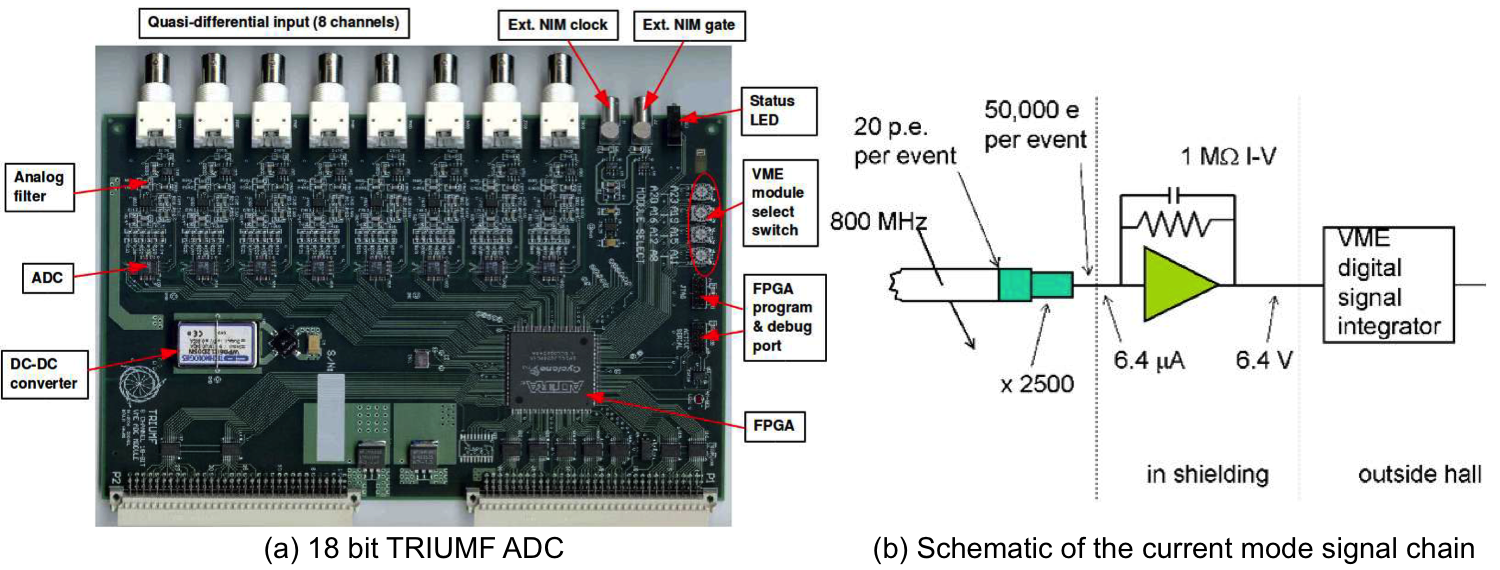
\includegraphics[width=15.0cm]{figures/adc}
	\caption
%	[Schematic of a TRIUMF made ADC and current mode signal chain.]
	{Schematic of a TRIUMF made ADC and current mode signal chain.}
	\label{fig:adc}
	\end{center}
\end{figure}
\end{singlespace}

\subsubsection{Low Noise Electronics\index{Main \v{C}erenkov Detectors!Low Noise Electronics}}%
\label{Low Noise Electronics}

Low noise current-voltage preamplifiers and digitizing integrators were designed and built by \newnot{symbol:TRIUMF}TRIUMF~\cite{website:TRIUMF} to minimize the contribution of electronic noise in the statistical uncertainty. The preamplifiers convert the DC anode current coming from the PMTs to a voltage $\sim$6~V signal for nominal production running. This signal is then digitized by 18-bit analog to digital converters (\newnot{symbol:ADC}ADCs\index{ADC}) at a sampling rate of 500~kHz to integrate at 1~kHz~\cite{manual_TRIUMF_ADC}. Each ADC module has eight ADC channels which were synchronized and triggered by the MPS signal from helicity board. A signal with 960~Hz event rate was integrated by summing the samples within the event window and then samples were stored in the channel memory on First-In-First-Out (FIFO) basis to avoid data loss due to delayed read-cycles. Another feature of this module was to produce the sum of the samples over four equal sub-blocks within an event. This sub-block feature of the ADCs was very useful to observe signal variations within an event for diagnostics. 


\subsubsection{Focal Plane Scanner\index{Main \v{C}erenkov Detectors!Focal Plane Scanner}}%
\label{Focal Plane Scanner}

A focal plane scanner was used to measure the beam profile in both high current production running and low current tracking mode in order to test systematic effects like target density change. Two 1~cm$\times$1~cm$\times$1~cm fused silica quartz radiator overlapped in a ``V" shaped and signals were read by individual PMTs in the scanner. This scanner system is then mounted on MD octant 7 (as shown in Figure~\ref{fig:main_detector} (b)) for beam profile scan. One example of such scan at 50~$\mu$A beam current with LH$_{2}$ target is shown in Figure~\ref{fig:main_detector} (d). J. Pan has described in details about the construction, schematic and analysis of focal plane scanner in her thesis~\cite{jie_qweak_thesis}.


\subsection{Luminosity Monitors\index{Luminosity Monitors}}%
\label{Luminosity Monitors}


The luminosity monitors (lumis), like the main detectors, were based on fused silica \v{C}erenkov radiators and with a light guide flushed with nitrogen gas to minimize corrosion. Two types of azimuthally symmetric luminosity monitors were used as beam diagnostic tools for the Q-weak experiment. The upstream luminosity monitors were located on the front face of the primary collimator 5~m from the target (shown in Figure~\ref{fig:lumi} (a)) and the downstream luminosity monitors are located 17~m downstream of the target and very close to the beam dump area (shown in Figure~\ref{fig:lumi} (b)). Both lumis were expected to detect electrons from small angle electron-proton and electron-electron scattering with an anticipated null asymmetry (ppb-level asymmetry). Upstream lumis were extremely useful for estimating beamline backgrounds. In some cases the measured asymmetry by the lumis were not as small as expected and and were also time dependent. Examples will be discussed in a later chapter. More detailed description of luminosity monitors and analysis can be found in J. Leacock's thesis~\cite{leacock_qweak}.


\begin{singlespace}
\begin{figure}[!h]
	\begin{center}
	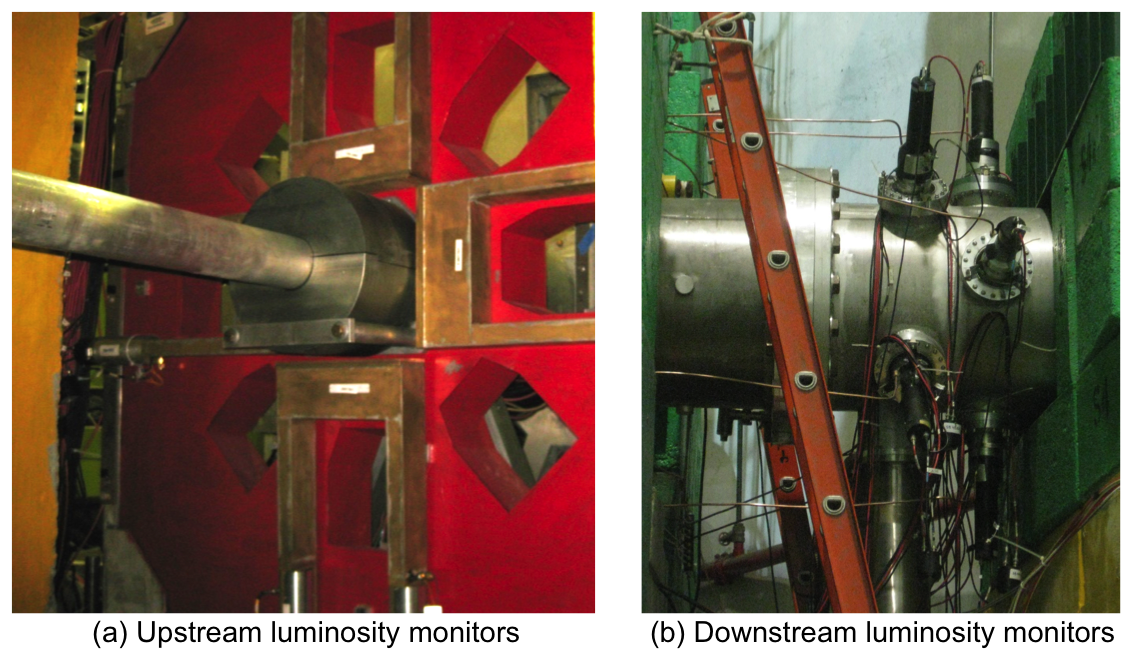
\includegraphics[width=15.0cm]{figures/lumi}
	\caption
%	[Luminosity monitors.]
	{Luminosity monitors. (a) Four upstream luminosity monitors installed on the face of the primary collimator. (b) Eight downstream luminosity monitors near beam dump.}
	\label{fig:lumi}
	\end{center}
\end{figure}
\end{singlespace}


\section{Tracking Detector System}%
\label{Tracking Detector System}

The asymmetry of the elastically scattered electron is approximately proportional to the four momentum transfer squared, $Q^{2}$ (details in Equation~\ref{equ:kinQ2}). A tracking system was necessary to measure $Q^{2}$ with 0.5\% relative uncertainty as proposed by the experiment (shown in Table~\ref{tab:qweak_proposal}). A pair of horizontal drift chambers (\newnot{symbol:HDC}HDCs) in region 2 (\newnot{symbol:R2}R2) were used to determine the scattering angle $\theta$ with an angle resolution of $\sim$0.6 $\mu$rad and particle trajectory with a position resolution $\sim$200~$\mu$m (as shown in Figure~\ref{fig:qweakApparatus}). Four set of vertical drift chambers (\newnot{symbol:VDC}VDCs) and two trigger scintillators were used upstream of the target (shown in Figure~\ref{fig:qweakApparatus}) in region 3 (\newnot{symbol:R3}R3) to measure $Q^{2}$ (more details in J. Lackey's thesis~\cite{lackey_qweak}). Detector packages in R2 and R3 can be rotated into each MD octant pair using a mechanical rotor to measure any octant dependence. Relation of $Q^{2}$ with $\theta$ is shown in Equation~\ref{equ:kinQ2}. The tracking system operated at $\sim$6 order of magnitude smaller beam current than parity production current. A details description of tracking system can be found in J. Pan's thesis~\cite{jie_qweak_thesis}.


%%%%%%%%%%%%%%%%%%%%%%%%%%%%%%%%%%%%%%%%%%%%%%%%%%%%%%%%%%%%%
\section{Data Acquisition}%
\label{Data Acquisition}

The Q-weak data acquisition (\newnot{symbol:DAQ}DAQ) system was based on the CEBAF Online Data Acquisition (\newnot{symbol:CODA}CODA)~\cite{website:CODA_wiki,Banta:1997ac} framework designed for experiments at Jefferson Lab. Two independent DAQ configurations were used for the experiment: integration mode for high current production data taking and counting mode for low current tracking measurements. The data taking during integration mode was triggered by the MPS signal from the accelerator with frequency of 960~\newnot{symbol:Hz}Hz and trigger scintillators were used as the trigger for the event mode running. A software prescale factor was used to control how often the DAQ was triggered by the specific trigger for each hardware trigger. Several read out controllers (\newnot{symbol:ROC}ROCs) were used to install different subsystem electronics. The CODA system used ethernet to communicate with all the ROCs. The Event Builder (\newnot{symbol:EB}EB) system was used to generate complete event from data fragments read from ROCs and the Event Transfer (\newnot{symbol:ET}ET) system provided central access to data events for multiple clients at real-time. The data rate during integration mode was approximately 5.6 MB/s. Data taken in an hour was defined as run and each run was segmented into 1.9 - 2.0~GB data files called runlets. One run has about 9 - 12 runlets. During the entire experiment $\sim$120~TB of raw data were collected. The averaged data such as yields, asymmetries, differences, HWP state, target, regression slopes, flags for data quality were saved to a MySQL database. 
B. Waidyawansa~\cite{buddhini_qweak} and R. Beminiwattha~\cite{rakitha_qweak} provided more technical details on data acquisition in their theses.


%%%%%%%%%%%%%%%%%%%%%%%%%%%%%%%%%%%%%%%%%%%%%%%%%%%%%%%%%%%%%
\section{Online Displays and Data Monitoring}%
\label{Online Displays and Data Monitoring}

The collected raw data files were processed to produce CERN ROOT and MySQL structured files for real time data quality monitoring and to store for future analysis. The real time analyzer produced a ROOT file for the first 100,000 events for each one hour production run. This ROOT file was used to generate all the necessary figures and summary tables to monitor the data quality and key physics parameters. Then C++, ROOT, and HTML\newnot{symbol:HTML} based analysis structure ${ \tt qwanalysis}$ with Hall-C wrapper script ${\tt hclog\_post}$~\cite{brads_communication} were used to produce HTML files and uploaded automatically to Hall-C electronic log book (HCLOG) for each run. A CODA trigger was used to initiate the analysis process when ROOT file generation for the first 100,000 events was completed. Necessary precautions and changes were made for the next run based on careful screening of standard acceptable set of parameters for the ongoing run.

One of the key component of the experiment was the target and was necessary to monitor it constantly. A C++ and Virtual Network Computing (\newnot{symbol:VNC}VNC) based software was used to monitor the target, and related parameters and to publish the status in the web. 
A snapshot of the target controls, all the key parameters, temperature from different sensors, cryogenic liquid flow, alarm handler, and cameras that monitors the target were taken every few minutes by the software and uploaded in the website~\cite{website:target}. This system was also used as a backup control system for the target in case of a failure of the computer that controlled the target. 
The same software, and technique were also used to monitor the beamline optics~\cite{website:bmod} for each production run by monitoring the BPM responses to the beam modulation signals and will be discussed in the later chapter. 

%%%%%%%%%%%%%%%%%%%%%%%%%%%%%%%%%%%%%%%%%%%%%%%%%%%%%%%%%%%%%
\section{Parity Analysis}%
\label{Parity Analysis}


To extract the main detector normalized yields for asymmetry calculations, several corrections applied on raw yields as described below.

\begin{equation} \label{equ:yieldDefinition}
Y^{+/-} = \frac{\displaystyle \frac{(Y_{\textrm{raw}}^{+/-} - Y_{\textrm{ped}})\times g}{N_{s}} }{I^{+/-}}
\end{equation}

where $Y_{\textrm{raw}}^{+/-}$ is the raw ADC signal in the ``+/-" helicity state, $Y_{\textrm{ped}}$ is the measured beam off signal or pedestal (a details pedestal analysis of the entire experiment is discussed in latter chapter), $g$ is the calibration factor to convert ADC counts per sample to volts, $N_{s}$ is the number of 2~$\mu$s read-out samples per MPS state, and $I^{+/-}$ beam is the beam current in the ``+/-" helicity state. 
The pedestals were subtracted from the raw signals to remove the effect from the DC offsets of the electronics chains, dark current due to thermal noise and cosmic rays.
In order to sum the two PMT signals for one detector to obtain the detector’s yield, or to sum the total 16 PMT signals to obtain the yield for all detectors, the gains of those PMT channels were matched to each other. 
The main detector yields are normalized to beam current to reduce the dependence on beam intensity fluctuations.
Beam stability cut is applied to the raw detector yield to eliminate data taken during a beam trip or unstable beam excursion~\cite{rakitha_qweak}. Further cuts to the data are made on a runlet-by-runlet basis during data quality checks. 
%Helicity correlated false asymmetries are then removed using linear regression techniques using natural beam jitter or driven beam modulation system.


The parity analysis engine processes raw data to extract event and pattern based quantities. Events which pass the event and pattern number checks are grouped into patterns of four events, known as quartets and the pattern based differences, yields, and asymmetries are computed as shown in Table~\ref{tab:variable_definition}. 
In the final step of the data analysis process, event and pattern based processed data were saved into a set of pre-defined histograms and ROOT trees. Event based yields are saved in the Mps\_Tree and pattern based differences, yields, and asymmetries are saved in the Hel\_Tree. Additionally, event based EPICs values for key components (QTOR current, target position, etc.) are stored in a Slow\_Tree. The running averages, running sums, uncertainties on the running averages and the slow control values are written into the MySQL databases.


\renewcommand{\arraystretch}{2.0} % make cell wider
\begin{singlespace}
\begin{table}[!h]
\begin{center}
  	\caption
%  	[Definition of different variables used in the experiment.]
  	{Definition of different variables used in the experiment~\cite{buddhini_qweak}. The subscripts indicate the event sequence in a quartet pattern defined as 1, 2, 3, 4 with helicity ``+$--$+". The definition of differences, yields, and asymmetries are shown here. Two different ways of combining yields and asymmetries were used in the experiment. The barsum yields are extracted using yields of the left/right PMTs ($Y_{L/R}$) with proper weights ($W_{L/R}$). The yields and asymmetries for each detector bar or for the whole detector were computed using the barsum yields and asymmetries. Another way to combine yields and asymmetries was pmtavg. The yield and asymmetry for each PMT were calculated first and then averaged to get yields and asymmetries for each detector or whole detector.}
  \begin{tabular}{ l | c | c }
%    \hline
    \noalign{\hrule height 1pt}
    Quantity 	& Definition & Comments\\ 
%    \hline
    \noalign{\hrule height 1pt}
	differences 	& $\displaystyle D = \frac{ (Y^{+}_{1}+Y^{+}_{4}) - (Y^{-}_{2}+Y^{-}_{3}) }{ 2 }$	& \parbox{5.0cm}{\centering BPMs, Combined BPMs, Energy calculator}\\
	\hline
	yields 		& $\displaystyle Y = \frac{ (Y^{+}_{1}+Y^{+}_{4}) + (Y^{-}_{2}+Y^{-}_{3}) }{ 2 }$ 	& \parbox{5.0cm}{\centering All detectors} \\ 
	\hline
	asymmetry 	& $\displaystyle A = \frac{ (Y^{+}_{1}+Y^{+}_{4}) - (Y^{-}_{2}+Y^{-}_{3}) }{ (Y^{+}_{1}+Y^{+}_{4}) + (Y^{-}_{2}+Y^{-}_{3}) }$ 	& \parbox{5.0cm}{\centering PMTs, Lumis, BCMs,BPM effective charge} \\
    \noalign{\hrule height 1pt}
	barsum 		& $\displaystyle Y_{\textrm{barsum}} = \frac{ W_{L}Y_{L}+W_{R}Y_{R} }{ W_{L}+W_{R} }$ 	&\parbox{5.0cm}{\centering $A_{\textrm{barsum}}$ calculated using yields} \\
	\hline	
	pmtavg 		& $\displaystyle A_{\textrm{pmtavg}} = \frac{ 1 }{ 2 }$($A_{L}+A_{R}$) 	& \parbox{5.0cm}{\centering $A_{L/R}$ is calculated from PMT yields}\\
	\hline		
	mdallbars 	& $\displaystyle Y_{\textrm{allbars}} = \frac{ 1 }{ 8 }$ $\sum_{i=1} Y_{\textrm{barsum}}^{i}$ 	& \parbox{5.0cm}{\centering $A_{\textrm{allbars}}$ calculated using yields} \\
	\hline	
	mdallpmtavg 	& $\displaystyle Y_{\textrm{pmtavg}} = \frac{ 1 }{ 16 }$ $\sum_{i=1}(Y_{L}^{i} + Y_{R}^{i})$	& \parbox{5.0cm}{\centering $A_{\textrm{pmtavg}}$ calculated using yields} \\
%	\hline
    \noalign{\hrule height 1pt}
  	\end{tabular}
  \label{tab:variable_definition}
\end{center}
\end{table}
\end{singlespace}
\renewcommand{\arraystretch}{1.0} % make cell wider




%
%A lower current cut of 100 μA was required3 to remove low
%current beam which were seen [41] to shift the ˇ Cerenkov detector asymmetries in a
%non-statistical way. The upper event cut on the BPM wires removes saturation which occurs during beam ramps and can cause false beam angles at the target. The lower
%event cut on the BPMs is used to remove events where a BPM can malfunction and
%produce noise which can be mistaken as position information.
%

%Events which pass the event and pattern number checks are grouped into
%patterns of four events, known as quartets and the pattern based asymmetries, differences
%and yields are computed as shown in Table 4.3. Additionally, for diagnostic
%purposes, there are several options (see Table 4.4 and Table 4.5) available to form the
%asymmetries and yields from the individual ˇ Cerenkov detectors and the full detector
%array. For all the pattern based asymmetries, yields and differences calculated from
%different detectors and beam monitors, a running average, a running sum and the
%error on the running average are also calculated in parallel using an algorithm developed
%by the Sandia National Laboratories [133] for statistical moment calculations of
%large scale data sets.



%During the final step of the analysis process, the analyzer saves the event based
%and pattern based processed data into a set of pre-defined histograms and ROOT
%trees. Event based yields are saved into the Mps Tree and pattern based asymmetries,
%average yields and the differences are saved into the Hel Tree. In addition, event based
%EPICs values are stored into a ROOT tree named Slow Tree. For diagnostics and
%quality checks, the configuration used by the analyzer and its version are also stored
%into the rootfile. Finally, the running averages, running sums, errors on the running
%averages and the slow control values (QTOR current, target position, etc.) read in
%via EPICS are written into the MySQL databases.

%(See Figure 6.1.) For the ˘ Cerenkov detectors and luminosity monitors, YR/L is proportional to the differential scattering cross section (see Appendix D.2) hence, the YR/L are used to compute the raw asymmetries from main detectors.
%
%A quartet (QRT) is defined to be one of two MPS patterns: L1,R1,R2,L2 or R1,L1,L2,R2 as discussed in Section 3.1. The raw asymmetry and average yield are computed for each QRT,


%Pedestal Subtraction The main detector consists of eight octants, and the yield 1 of each detector is recorded by two PMT channels. The pedestals of those channels, i.e. the DC offsets of the electronics chains, including dark current due to thermal noise and cosmic rays, must be subtracted from the raw signals so that real detector yields can be obtained. The pedestals may change periodically due to variations in temperature, room backgrounds, etc. To account for these effects, brief pedestal runs are taken once or twice per day with beam off during production data taking. The average pedestal values are subtracted from the yield of each PMT channel. The subtraction is done with the most recently updated pedestal values.
%
%PMT Gain Match The light yield seen by one PMT decreases with distance from the PMT along the quartz bar. The sum of the two PMTs’ light yields exhibits reduced position dependence. In order to sum the two PMT signals for one detector to obtain the detector’s yield, or to sum the total 16 PMT signals to obtain the yield for all detectors, the gains of those PMT channels should be well matched to each other. The gain is adjusted by adjusting each PMT’s high voltage. Weighting factors are used in the analysis software to further equalize the PMTs’ yields. These factors are determined based on weighting each PMT’s yield by the average yield of 16 PMTs taken from a good quality production run.
%
%Beam Current Normalization In order to reduce the dependence on beam intensity fluctuations, the main detector yields are normalized to beam current (or beam charge) after pedestal subtraction. The normalization is done in each MPS according to a particular BCM’s readout. BCMs are calibrated periodically in dedicated runs.
